\documentclass{article}

% Submission option (default = double-blind Main Track)
\usepackage{neurips_2026}

\usepackage[utf8]{inputenc}
\usepackage[T1]{fontenc}
\usepackage{hyperref}
\usepackage{url}
\usepackage{booktabs}
\usepackage{amsfonts}
\usepackage{amsmath}
\usepackage{amssymb}
\usepackage{nicefrac}
\usepackage{microtype}
\usepackage{xcolor}
\usepackage{graphicx}
\usepackage{multirow}
\usepackage{array}
\usepackage{placeins}

\title{The Missing Positional Story in LLMs: A Case Study of Shift-Invariant Attention}

\author{%
  Benjamin Huh \\
  Dartmouth College \\
  \texttt{benjamin.j.huh.24@dartmouth.edu}
  \And
  Hak Hyun Kim \\
  Dartmouth College \\
  \texttt{hak.hyun.kim.gr@dartmouth.edu}
  \And
  Yuting Tian \\
  Dartmouth College \\
  \texttt{yuting.tian.th@dartmouth.edu}
  \And
  Jason Peng \\
  Dartmouth College \\
  \texttt{jason.peng.23@dartmouth.edu}
  \And
  Christopher Kang \\
  Dartmouth College \\
  \texttt{christopher.kang.26@dartmouth.edu}
  \AND
  Soroush Vosoughi (PI) \\
  Dartmouth College \\
  \texttt{soroush.vosoughi@dartmouth.edu}
}

\begin{document}

\maketitle

\begin{abstract}
Rotary positional embeddings (RoPE) are now the dominant positional mechanism in modern large language models. By construction, RoPE encodes a shift-invariant (SI) channel in attention: head logits can depend purely on token offset rather than absolute position. We show that trained models do not just inherit this SI channel; they actively learn to exploit it. This exploitation is load-bearing: SI ablations produce systematic degradation that tracks per-head SI amplitude under converging specificity controls, and SI structure appears even in models trained with absolute positional encodings, indicating that this is learned computation rather than a purely architectural artifact. This SI exploitation is also functionally meaningful: SI ablation preferentially disrupts offset-structured retrieval, most robustly in Llama and Mistral, with directional extension to naturalistic long-context settings. At the same time, our results surface a deeper question: is the SI channel currently underutilized? Many computations are position-invariant by nature --- recognizing that a pattern holds regardless of where it appears in context --- yet our evidence suggests current models allocate SI channels mostly to narrow positional and surface routing rather than these richer invariances. Strikingly, SI exploitation amplitude varies more than sixfold, a spread that holds across eleven models spanning seven architecture families, indicating that degree of SI use is a trainable property rather than an architectural given. This points to a practical direction: pretraining pressure toward semantic invariance tasks may push models to exploit SI channels for richer computation than what we observe today.
\end{abstract}

\section{Introduction}

Whether attention heads develop computations that are stable across token positions---robust to \emph{where} in context a pattern appears, not just \emph{what} the pattern is---matters for long-context reasoning, in-context learning, and retrieval.
Transformer attention \citep{vaswani2017attention} combined with rotary positional embeddings (RoPE) \citep{su2021roformer}, now the dominant positional mechanism in modern large language models, gives each head an architectural route to this property: query--key inner products under rotary transformations can depend purely on the \emph{difference} in token positions rather than their absolute values.
We call this the \emph{shift-invariant} (SI) channel.
Its existence is guaranteed by RoPE's geometry.
What trained models actually do with it---whether they exploit it, how load-bearing that exploitation is, and how heterogeneous it is across architectures---has not been systematically studied.

This paper addresses those questions.
We show that trained 7--8B RoPE models do not passively inherit the SI channel; they actively exploit it in structured, load-bearing ways.
We operationalize per-head SI strength as the fraction of attention logit variance explained by an offset-only function ($R_h^2$), and intervene by subtracting the estimated SI kernel from selected heads at evaluation time.
The central finding is a dose-response relationship: head-level disruption cost scales monotonically with $R_h^2$ under a converging set of specificity controls---permutation controls, importance-matched non-SI baselines, and kernel-transplant tests---ruling out generic head importance and local-bias artifacts as explanations.
A constant-offset control, invariant under softmax, confirms that position-specificity of the learned kernel, not its magnitude, drives the effect.

The motivating empirical observation is that SI exploitation is highly heterogeneous.
Across three primary RoPE models, mean per-head $R^2$ spans 6.5$\times$ (Llama-3.1-8B: 0.380; Mistral-7B: 0.266; OLMo-2-7B: 0.058).
A proxy-scale multi-seed variance decomposition confirms this spread reflects genuine between-model differences rather than training-run noise.
A breadth consolidation across 11 models spanning 7 architecture families extends the spread to 140$\times$ max/min---and, strikingly, GPT-2 models trained with absolute positional encodings show non-trivial SI structure, establishing that SI exploitation is learned computation rather than a consequence of RoPE geometry alone.
Degree of SI use is therefore a trainable property, not an architectural given, which points toward pretraining design as a lever for amplifying or redirecting it.

SI exploitation is also functionally meaningful.
Targeted ablation of high-SI heads preferentially disrupts offset-structured retrieval relative to matched controls, most robustly in Llama and Mistral.
Transfer boundaries are explicit: sensitivity narrows under stricter format controls and broader probe families, and extends directionally to naturalistic long-context settings in the two high-SI models.
Two interpretive lenses organize these findings.
A \textit{frequency-domain lens} connects the oscillatory structure of learned SI kernels to their intervention cost: richer spectral content in a head's learned kernel predicts larger disruption, providing a mechanistic link between kernel shape and load-bearing capacity (Appendix~B).
A \textit{representational-commitment hypothesis} frames current SI allocation as dominated by narrow positional and surface routing, with broader semantic invariance under-realized and representing a tractable pretraining target.

\paragraph{Contributions.}
\begin{enumerate}
\item \textbf{Head-level SI specificity} (primary result): per-head $R_h^2$ is a strong predictor of disruption cost under SI-kernel ablation, confirmed by permutation, importance-matched, kernel-transplant, and local-bias controls across three 7--8B models (Section~\ref{sec:headlevel}).
\item \textbf{Bounded functional sensitivity}: SI-targeted ablation preferentially disrupts offset-structured retrieval, with transfer scope explicitly characterized across controlled, format-matched, synthetic, and naturalistic long-context settings (Section~\ref{sec:functional}).
\item \textbf{Cross-model heterogeneity}: SI exploitation amplitude spans 140$\times$ across 11 models and 7 architecture families; the spread is real (not seed noise) and appears in non-RoPE architectures, establishing SI exploitation as a trainable property (Section~\ref{sec:headlevel}; Appendix~L).
\end{enumerate}

\paragraph{Terminology.}
We use \textit{load-bearing} to mean that an intervention on a measured component causes reliable performance degradation, and \textit{robustness controls} for post-hoc checks that bound confounds and scope.


\section{Related Work}

\paragraph{RoPE, positional structure, and offset-conditioned computation.}
Prior work shows that positional encoding choices shape what attention heads can represent \citep{vaswani2017attention,shaw2018self,press2022train,su2021roformer}. RoPE makes relative-offset structure especially accessible, and context-extension studies (e.g., PI and YaRN) analyze how frequency bands contribute to positional behavior \citep{chen2023extending,peng2023yarn}. Our focus is different: we measure per-head offset-conditioned structure and test whether that structure is load-bearing under targeted intervention, extending descriptive positional analyses \citep{barbero2024round}.

\paragraph{Head specialization, mechanistic intervention, and retrieval behavior.}
Head-level specialization and pruning work shows that some heads are functionally important while others are redundant \citep{clark2019analyzing,voita2019analyzing,michel2019sixteen,conmy2023acdc}. Mechanistic tools such as activation patching, causal tracing, and causal scrubbing motivate intervention-based attribution \citep{meng2022locating,chan2022causal}. Induction-head and long-context retrieval literature highlights offset-structured behaviors that may rely on sparse head populations \citep{elhage2021framework,olsson2022context,wu2024retrieval,xiao2023efficient}. We build on these threads with an SI-specific intervention stack, separating strong head-level specificity evidence from weaker collective and transfer-level evidence, and with a broader multi-model heterogeneity consolidation.

\paragraph{What prior work does not yet resolve.}
Existing positional and interpretability studies do not jointly answer three questions that are central here: whether SI-attributed structure is load-bearing under controlled intervention, where functional transfer boundaries lie beyond aligned toy settings, and how heterogeneous SI exploitation is across model families under a common measurement protocol. Our design targets this combined gap directly by pairing head-level intervention specificity tests with bounded functional probes and a multi-family heterogeneity consolidation.

\section{Setup}

\begin{figure}[htbp]
\centering
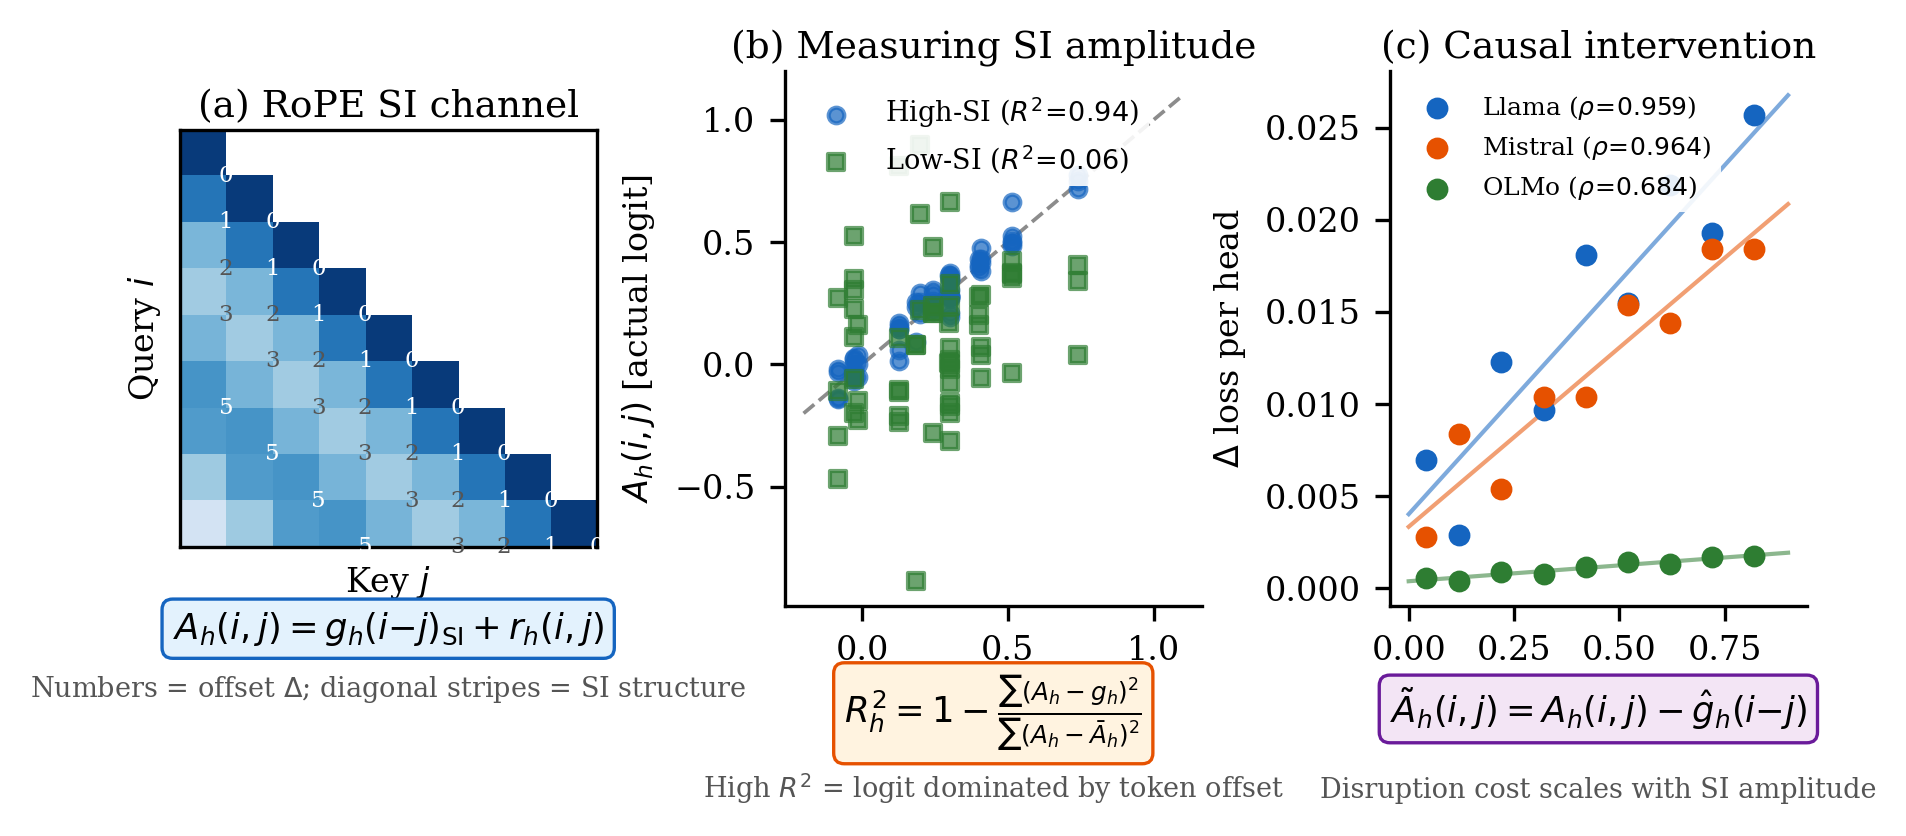
\includegraphics[width=0.86\textwidth]{../neurips2026/figures/fig_overview_schematic.png}
\caption{Overview of the SI channel, measurement, and intervention. \textbf{(a)} Pre-softmax attention logits decompose into an offset-only component $g_h(i{-}j)$ (shift-invariant) and a residual $r_h(i,j)$; diagonal stripes in the attention matrix reflect SI structure. \textbf{(b)} $R_h^2$ measures the fraction of logit variance explained by $g_h$; high-SI heads (blue) cluster near the identity line, low-SI heads (green) scatter widely. \textbf{(c)} Subtracting $\hat{g}_h$ from head logits at evaluation time reveals that disruption cost scales monotonically with $R_h^2$, establishing the dose-response relationship that anchors the primary finding.}
\label{fig:overview}
\end{figure}

\subsection{SI operationalization}
For each head $h$, we decompose pre-softmax attention logits as
\begin{equation}
A_h(i,j) = g_h(i-j) + r_h(i,j),
\end{equation}
where $g_h(\Delta)$ is an offset-only component estimated nonparametrically by empirical means over all token pairs with $i-j=\Delta$. We score SI strength by
\begin{equation}
R_h^2 = 1 - \frac{\sum_{i,j}(A_h(i,j)-g_h(i-j))^2}{\sum_{i,j}(A_h(i,j)-\bar A_h)^2}.
\end{equation}
High-SI heads are the top quartile of $R_h^2$ within each model. Within-model rank designation is complemented by absolute-threshold robustness checks (Appendix~\ref{app:running}): the rank-based disruption result replicates at every tested absolute threshold in the range $[0.15, 0.40]$, and per-head disruption at $T{=}0.20$ tracks model-level mean $R^2$ across all three models.

\paragraph{What $R^2$ does and does not identify.}
Because offset bins are frequency-imbalanced and content-position correlations can exist in natural corpora, this $R^2$ identifies \emph{in-distribution} SI exploitation rather than corpus-free architectural SI. Pairwise weighting means common short offsets dominate the fit, while large-offset estimates are noisier due to lower support. Since $R^2$ is variance-normalized, cross-model contrasts are triangulated with intervention deltas in Section~4; absolute nats can vary with baseline entropy, so we also report percent and control-normalized sensitivity axes (Appendix~L). Two robustness checks directly target this limitation: offset-reweighting analyses reduce short-offset dominance, and corpus-transfer scoring evaluates stability across shifted text distributions. Both preserve cross-model ordering with bounded effect-size drift (Appendix~L), which narrows but does not eliminate the threat.

A key alternative interpretation is that high $R^2$ may partly reflect local-distance attention bias rather than richer SI computation. We therefore treat $R^2$ as an offset-conditioned structure score, not a standalone mechanism identifier. Local-bias decomposition controls show model-conditional support for non-trivial excess beyond simple local-decay nulls: disruption tracks $R^2_{\text{excess}}$ over a local-decay fit in Llama ($\rho{=}0.893$, $p{=}1.2{\times}10^{-7}$) and Mistral ($\rho{=}0.812$, $p{=}1.4{\times}10^{-5}$), but not in OLMo ($\rho{=}0.206$, $p{=}0.38$), which narrows but does not eliminate this ambiguity.

\subsection{Intervention}
We intervene at evaluation time by subtracting the estimated SI kernel from selected heads:
\begin{equation}
\tilde A_h(i,j) = A_h(i,j) - \hat g_h(i-j).
\end{equation}
This intervention targets the offset-only pre-softmax component while leaving residual logits unchanged before softmax. Because subtraction is position-dependent, downstream attention can redistribute non-trivially through softmax renormalization. We therefore interpret measured effects as \emph{intervention sensitivity signatures}: evidence that offset-conditioned structure is load-bearing under this perturbation class, not a full causal decomposition of redistribution pathways.

A constant-offset perturbation control provides direct evidence that position-specificity---not merely the magnitude of the kernel shift---is the load-bearing property. Applying a position-independent scalar equal to $\text{mean}(\hat{g}_h)$ per head preserves rank order and is invariant under softmax, so in theory it should not change LM loss. Empirically, this control leaves loss essentially unchanged in all three primary models: $\Delta \text{loss} = 0.00011$ nats (Llama; ratio $2913\times$ vs.\ true SI subtraction), $2.7\times10^{-5}$ nats (Mistral; ratio $21968\times$), and $-0.00017$ nats ($\approx 0$; OLMo, where both effects are near-zero consistent with low SI amplitude). In this local control setting, true SI subtraction causes losses of $+0.320$, $+0.592$, and $+0.015$ nats respectively; Section~4 reports larger values for the main ranked-head intervention protocol. This confirms that position-specificity of the kernel---not merely the norm of the shift---drives the disruption effect across all tested models.

An entropy analysis of high-SI heads provides complementary evidence on the redistribution pathway. True SI subtraction concentrates attention (mean head-entropy change $-0.887$ nats in Llama, $-0.719$ nats in Mistral), while permuted-kernel subtraction leaves entropy approximately unchanged ($+0.031$ and $-0.110$ nats); in OLMo the changes are small in both arms ($-0.064$ vs.\ $-0.029$ nats), consistent with the lower SI amplitude. The concentration pattern in Llama and Mistral is consistent with attention-sink absorption of redistributed attention when position-specific routing is removed. Full redistribution analysis tables are in Appendix~D. Importance-matched, permutation, transplant, and local-bias controls further reduce key alternatives.

\subsection{Models and evidence policy}
Primary models are Llama-3.1-8B \citep{dubey2024llama3}, Mistral-7B-v0.1 \citep{jiang2023mistral}, and OLMo-2-7B \citep{groeneveld2024olmo}. Llama and Mistral provide the strongest SI signal (mean $R^2$: 0.380, 0.266), while OLMo is a weak-SI anchor (0.058). Additional anchors (GPT-2-small/medium, TinyLlama-NoPE, Gemma) are used for scope and breadth checks, not matched-scale causal attribution.

The main intervention subtracts estimated SI kernels from selected heads and evaluates four specificity checks: permutation controls, importance-matched non-SI baselines, kernel-transplant checks, and local-bias decomposition. Main-text results focus on effect sizes and cross-model consistency; extended controls are reported in Appendix~\ref{app:running}.

\begin{figure}[htbp]
\centering
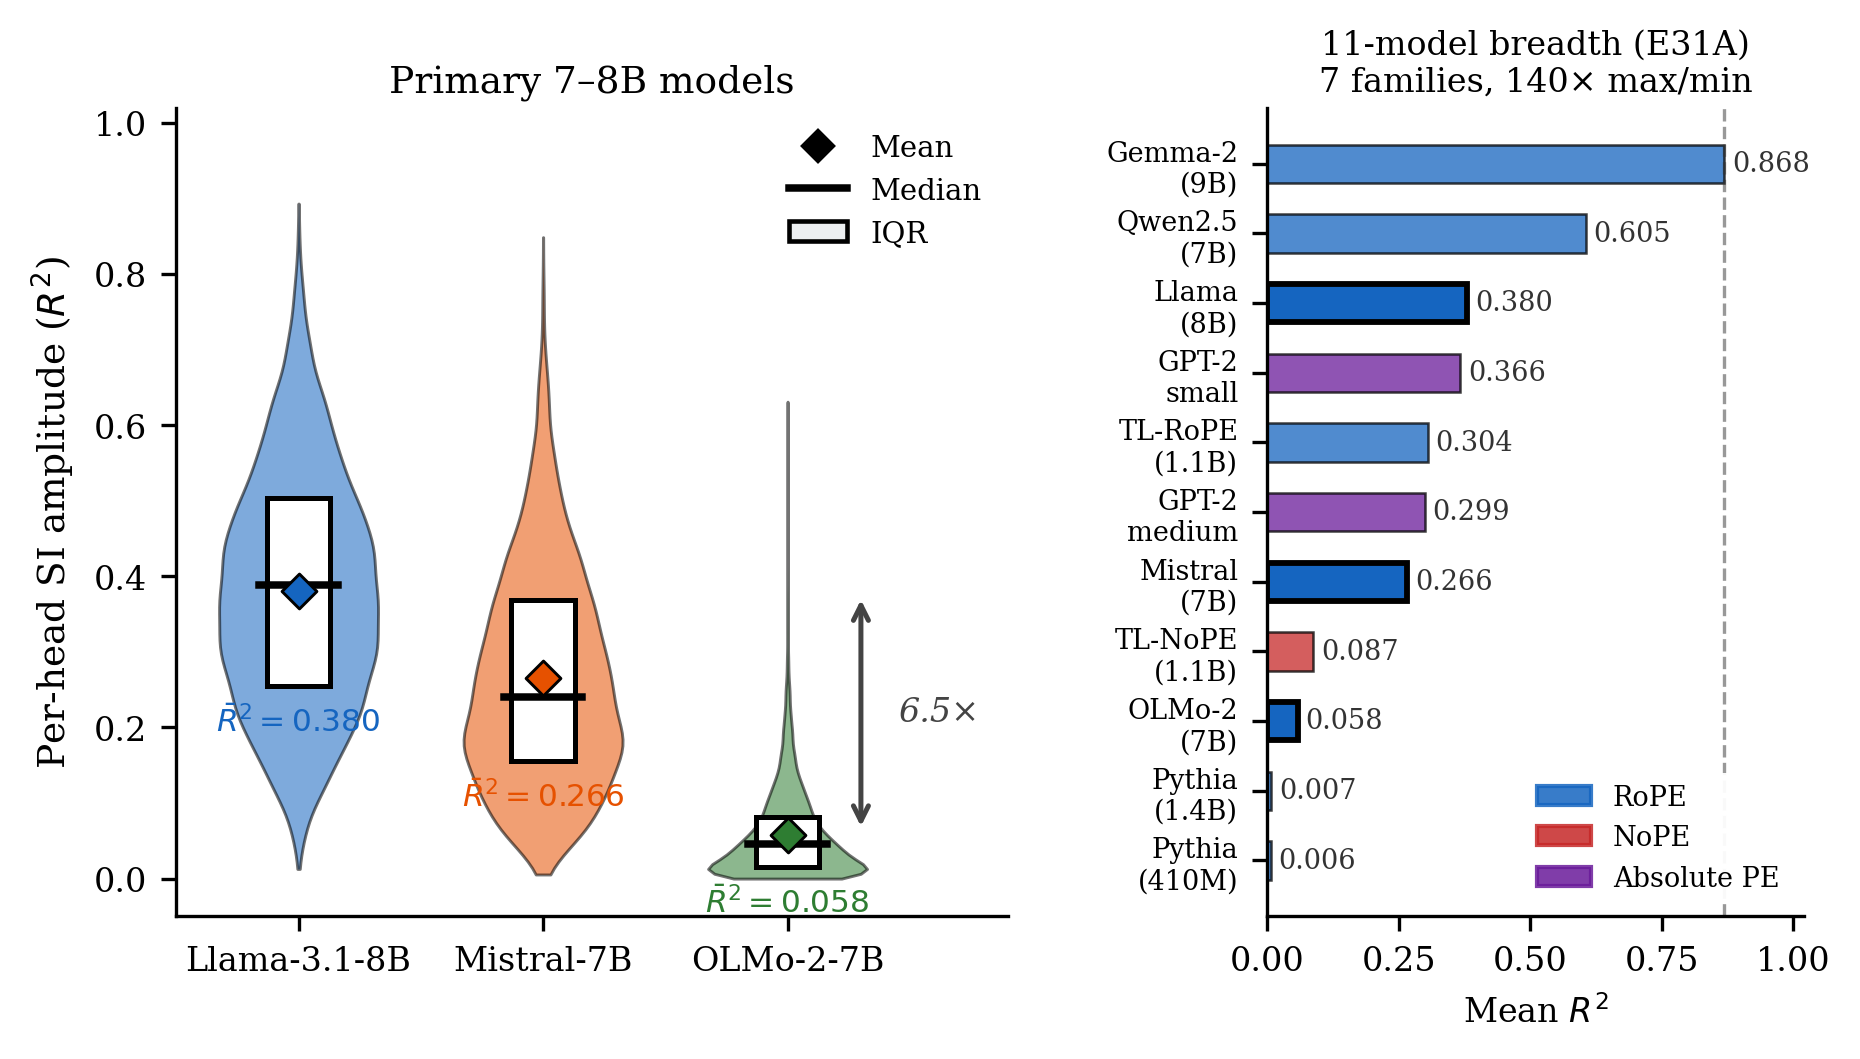
\includegraphics[width=0.88\textwidth]{../neurips2026/figures/fig_r2_heterogeneity.png}
\caption{SI exploitation amplitude varies widely across models. \textbf{Left}: per-head $R^2$ distributions for the three primary 7--8B models (violin = full distribution; box = IQR; line = median; diamond = mean). Cross-model spread is 6.5$\times$ (mean $R^2$: Llama 0.380, Mistral 0.266, OLMo 0.058). \textbf{Right}: mixed-scale breadth consolidation across 11 models spanning 7 architecture families (1.1B--9B); mean-$R^2$ range 0.006--0.868 (140$\times$ max/min). Pythia models anchor the minimum end; TinyLlama-NoPE is a low-SI NoPE control above that minimum; GPT-2 models (absolute PE, purple) show non-trivial SI, indicating this is learned computation rather than a RoPE-only artifact.}
\label{fig:setup_capacity}
\end{figure}

\section{Head-Level Shift Invariance Under Intervention}
\label{sec:headlevel}

\textbf{Head-Level Shift Invariance} is the main empirical result: SI intervention damage is load-bearing and systematically stratified by per-head SI amplitude. The most decisive specificity checks are permutation controls, importance-matched non-SI baselines, and kernel-transplant tests, with local-bias decomposition providing additional model-conditional support.

RoPE-equipped models exhibit non-trivial SI structure with a large cross-model range (mean $R^2$: Llama 0.380, Mistral 0.266, OLMo 0.058). At 1.1B proxy scale, TinyLlama-NoPE shows early-layer $R^2<0.01$; this proxy early-layer signal is distinct from TinyLlama-NoPE's full-model mean ($R^2{=}0.0868$). We treat the proxy result as weak directional capacity evidence only, not a matched 7--8B causal positional-family contrast. Because $R^2$ is a ratio, we interpret this spread jointly with absolute disruption deltas below rather than as a standalone measure of absolute SI magnitude. An expanded, mixed-scale breadth consolidation spanning all tested models---the three primary models plus eight additional architectures across four further families (Gemma-2-9B; Qwen2.5-7B; GPT-2-small, GPT-2-medium; TinyLlama-1.1B-RoPE, TinyLlama-1.1B-NoPE; Pythia-1.4B, Pythia-410M); 11 models total, 7 families; Appendix~L---shows mean-$R^2$ values ranging from 0.006 to 0.868 (max/min ratio $140\times$), reinforcing that SI exploitation amplitude is broadly heterogeneous across architectures and training regimes.

Under the main ranked-head SI intervention protocol (distinct from the local control-setting magnitudes in Section~3), LM loss increases by $+4.15$ nats in Llama (+206\%, $d=11.6$), $+3.43$ in Mistral (+185\%, $d=14.6$), and $+0.058$ in OLMo (+2.8\%, $d=0.81$). Permutation-specificity contrasts are positive in all three models (true-minus-permuted: Llama $+3.2774$, Mistral $+3.1926$, OLMo $+0.0427$; one-sided bootstrap $p=2.0\times10^{-4}$ each), indicating disruption cost specific to correct-offset structure rather than arbitrary offset subtraction.

Norm-matched perturbation controls (Appendix~L) place an upper bound on this effect: in all three models, true subtraction exceeds the permuted control but is weaker than norm-matched random perturbation. We therefore frame this finding as permutation-specific disruption cost that is load-bearing under intervention, bounded above by equal-norm random perturbation.

GPT-2 anchors (absolute PE) still show measurable SI structure (Figure~\ref{fig:setup_capacity}), indicating SI behavior is learned rather than a RoPE-only artifact. OLMo-only checkpoint trajectory analyses and toy-model causal probes are retained in Appendix~D/M as non-central context.\footnote{Exploratory toy-model causal probes are reported in Appendix~\ref{app:e23}; they provide future-work motivation but are not scale-matched primary evidence for the main-paper claims.}

\begin{figure}[htbp]
\centering
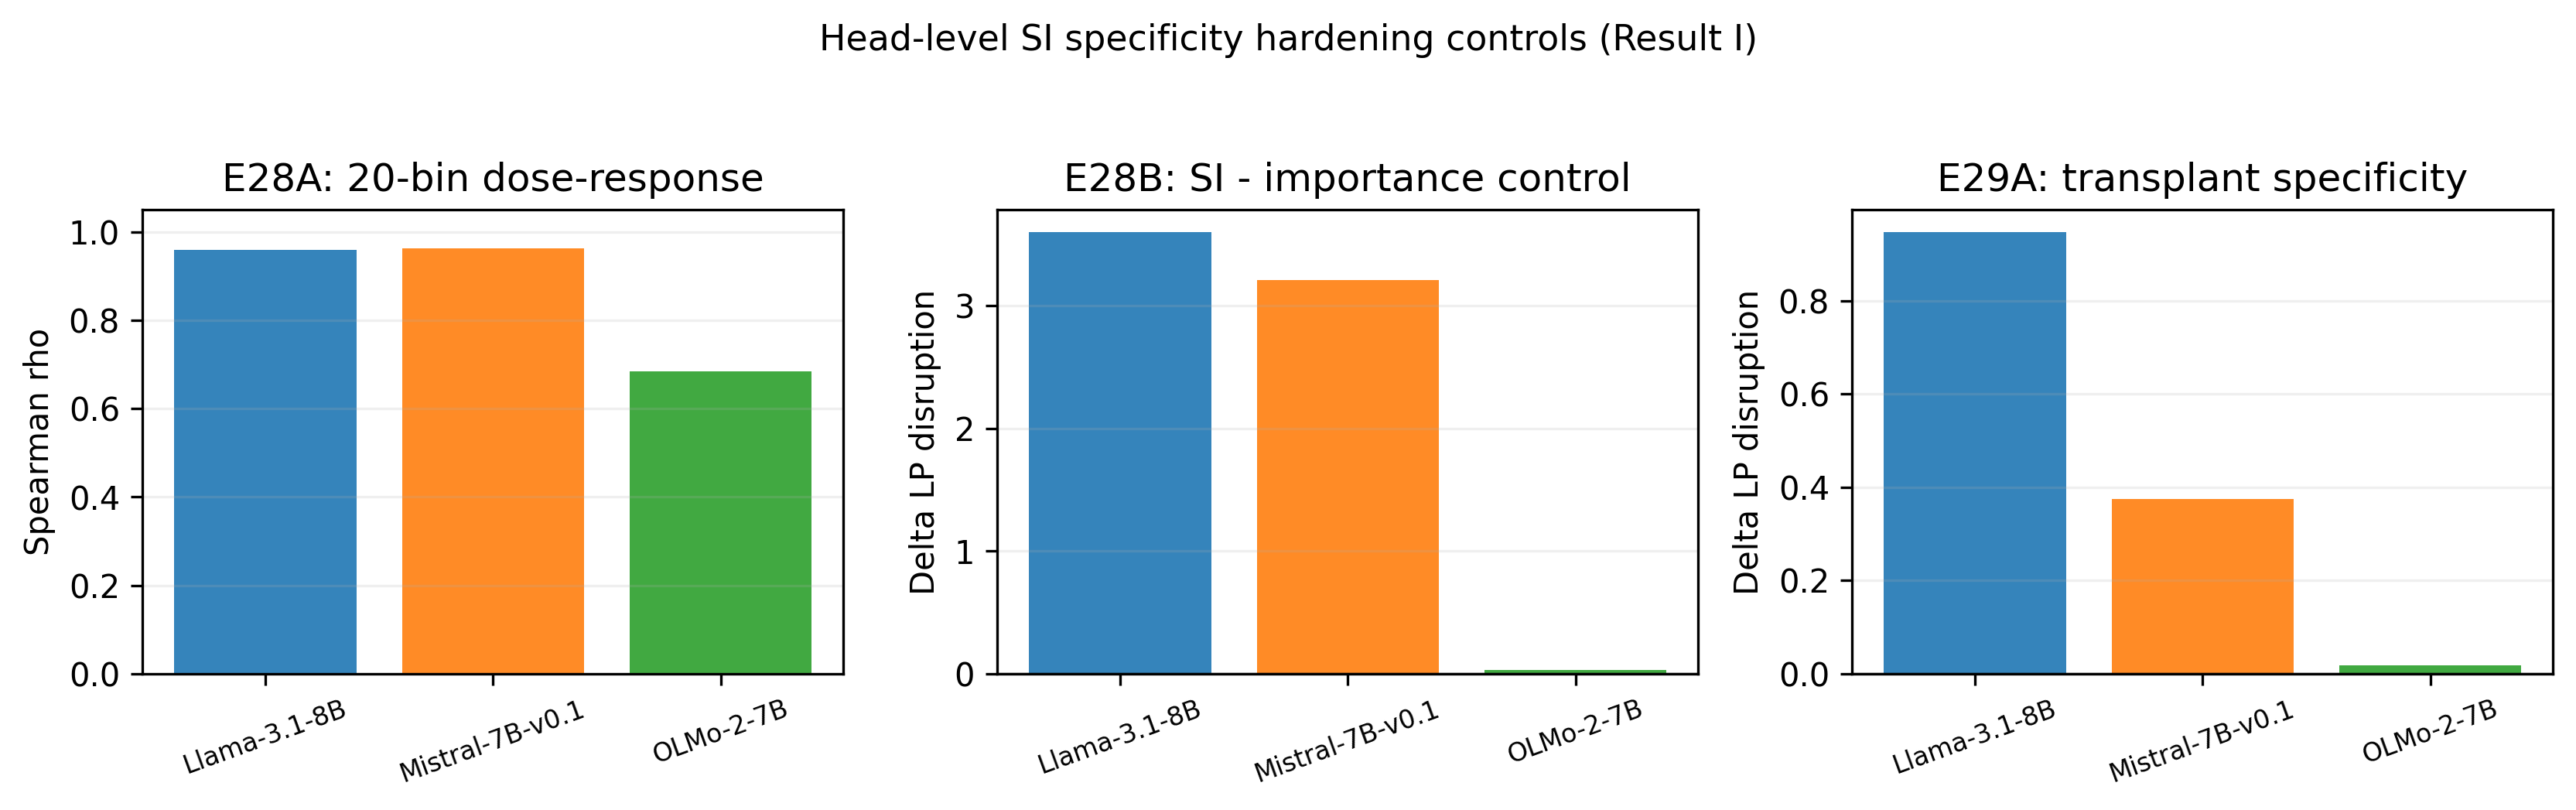
\includegraphics[width=0.94\textwidth]{../neurips2026/figures/fig_dose_response_controls.png}
\caption{Head-level dose-response and specificity controls (primary finding). \textbf{Left}: 20-bin Spearman correlation between per-head $R^2$ and disruption cost under SI-kernel subtraction (Llama $\rho{=}0.959$, Mistral $\rho{=}0.964$, OLMo $\rho{=}0.684$; all one-tailed permutation $p < 0.001$). \textbf{Center}: SI-ranked intervention minus importance-matched non-SI intervention (positive in all three models, ruling out generic head-importance as the driver). \textbf{Right}: Kernel-transplant specificity --- transplanting norm-matched high-SI kernels onto low-SI heads versus low-head self-subtraction (positive in all three models).}
\label{fig:dose_response}
\end{figure}

\begin{table}[htbp]
\centering
\scriptsize
\setlength{\tabcolsep}{3pt}
\caption{Head-Level Shift Invariance: model-by-model specificity summary. Each row is one model; columns report (i) head-level dose-response correlation, (ii) excess disruption of SI-ranked vs.\ importance-matched non-SI ablation, (iii) excess disruption of kernel transplant vs.\ low-head self-ablation, and (iv) whether the local-bias decomposition passes. Positive deltas indicate stronger SI-specific disruption.}
\label{tab:result1_hardening_snapshot}
\begin{tabular}{lcccc}
\toprule
Model &
\begin{tabular}[c]{@{}c@{}}Dose-response\\$\rho$\end{tabular} &
\begin{tabular}[c]{@{}c@{}}$\Delta$ vs matched\\non-SI (nats)\end{tabular} &
\begin{tabular}[c]{@{}c@{}}$\Delta$ transplant\\vs self (nats)\end{tabular} &
\begin{tabular}[c]{@{}c@{}}Local-bias\\check\end{tabular} \\
\midrule
Llama & 0.959 & +3.60 & +0.947 & pass \\
Mistral & 0.964 & +3.21 & +0.374 & pass \\
OLMo & 0.684 & +0.0267 & +0.0174 & fail \\
\bottomrule
\end{tabular}
\end{table}

\paragraph{Head-level dose-response and specificity controls (Figure~\ref{fig:dose_response}).}
The control stack is consistent across models: permutation specificity is positive in all three, SI-ranked intervention exceeds importance-matched non-SI baselines (SI-minus-importance-matched deltas: $+3.60$, $+3.21$, and $+0.027$ nats in Llama, Mistral, and OLMo respectively), and kernel-transplant controls show that transplanting high-SI kernels onto low-SI heads is more disruptive than low-head self-subtraction. Local-bias decomposition remains model-conditional (Llama/Mistral supported, OLMo non-pass). The 20-bin dose-response is positive in all three models (Llama $\rho=0.959$, Mistral $\rho=0.964$, OLMo $\rho=0.684$; all one-tailed permutation $p<0.001$). Absolute-threshold robustness and multi-axis comparability details are reported in Appendix~\ref{app:running}.

\section{Bounded Functional Sensitivity Under Offset-Structured Probes}
\label{sec:functional}

\begin{table}[htbp]
\centering
\scriptsize
\setlength{\tabcolsep}{3pt}
\caption{Bounded functional sensitivity summary. \textbf{Panel A} reports the core controlled-probe effect at model level. \textbf{Panel B} reports transfer scope across progressively stricter settings. Positive preferential gaps indicate larger SI-ablation damage in offset-structured conditions than matched controls.}
\label{tab:functional_summary}
\begingroup
\renewcommand{\arraystretch}{1.08}
\noindent\begin{minipage}{\columnwidth}
\centering
\textbf{Panel A: Controlled offset-repetition probe (core quantitative effect)}\\[2pt]
\begin{tabular}{@{}lcccc@{}}
\toprule
Model &
\begin{tabular}[c]{@{}c@{}}Offset-rep\\acc.\ $\Delta$\end{tabular} &
\begin{tabular}[c]{@{}c@{}}Matched-ctrl\\acc.\ $\Delta$\end{tabular} &
\begin{tabular}[c]{@{}c@{}}Preferential\\acc.\ gap\end{tabular} &
\begin{tabular}[c]{@{}c@{}}Preferential\\lp gap\end{tabular} \\
\midrule
Llama-3.1-8B & 0.910 & $-0.005$ & +0.915 & +8.509 \\
Mistral-7B-v0.1 & 0.715 & $-0.005$ & +0.720 & +6.767 \\
OLMo-2-7B & 0.345 & $-0.055$ & +0.400 & +4.575 \\
\bottomrule
\end{tabular}
\end{minipage}
\vspace{4pt}
\noindent\begin{minipage}{\columnwidth}
\centering
\textbf{Panel B: Transfer boundary scope (where the effect persists)}\\[2pt]
\begin{tabular}{@{}>{\raggedright\arraybackslash}p{2.8cm}>{\centering\arraybackslash}p{1.1cm}>{\raggedright\arraybackslash}p{3.7cm}@{}}
\toprule
Setting & Model passes & Interpretation \\
\midrule
Controlled offset-repetition probe & 3/3 & Strongest and most consistent setting. \\
Strict format-matched variant & 1/3 & Sensitive to demonstration-format confounds. \\
Broader synthetic probe families & 0/3 & No model-level transfer pass. \\
Natural-text long-context extension & 2/3 & Positive in Llama/Mistral, negative in OLMo. \\
2$\times$2 context/regularity boundary grid & 2/3 & Same split as natural-text extension. \\
\bottomrule
\end{tabular}
\end{minipage}
\endgroup
\end{table}

This section is a tightly scoped mechanistic sensitivity probe, not a naturalistic long-context ICL benchmark. Table~\ref{tab:functional_summary} Panel A reports the core controlled-probe effect: SI intervention is directionally more damaging for offset-repetition conditions than matched controls in all three models, with preferential accuracy gaps of $+0.915$ (Llama), $+0.720$ (Mistral), and $+0.400$ (OLMo), and preferential log-probability gaps of $+8.509$, $+6.767$, and $+4.575$. Table~\ref{tab:functional_summary} Panel B summarizes transfer boundaries: semi-naturalistic long-context probe families (wiki/code passkey contexts 256--512; Appendix~L) are positive in Llama and Mistral but negative in OLMo (2/3 model directional passes), and the 2$\times$2 context/regularity boundary grid reproduces the same split. We therefore promote this as a directional preferential-degradation result under intervention with explicit transfer boundaries, not as a stable scalar-ratio claim.

Strict format-confound controls are mixed/model-conditional (1/3 strict survival).\footnote{Strict format controls replace offset-repetition demonstrations with random-order demonstrations matched for token count; survival requires the preferential gap to persist under this swap.} Broader 7-family synthetic transfer is non-passing at model level (0/3).\footnote{The 7 probe families span offset-regularity and context-length combinations (full grid in Appendix~L); a model passes if $\geq$5/7 families show directional preferential disruption.} A two-model natural-text long-context extension (Llama and Mistral; 60 prompts each; Appendix~L) shows the same directional effect: SI-targeted ablation exceeds importance-matched non-SI ablation by $+3.64$ nats in Llama and $+3.12$ nats in Mistral (95\% CI $[2.21,\,4.04]$, one-sided permutation $p{=}3.3{\times}10^{-5}$). Taken together, these checks indicate a clear boundary: sensitivity is strongest when probes preserve explicit offset-structured retrieval under contextual distraction, and weakens under broader synthetic family diversity.

\begin{figure}[htbp]
\centering
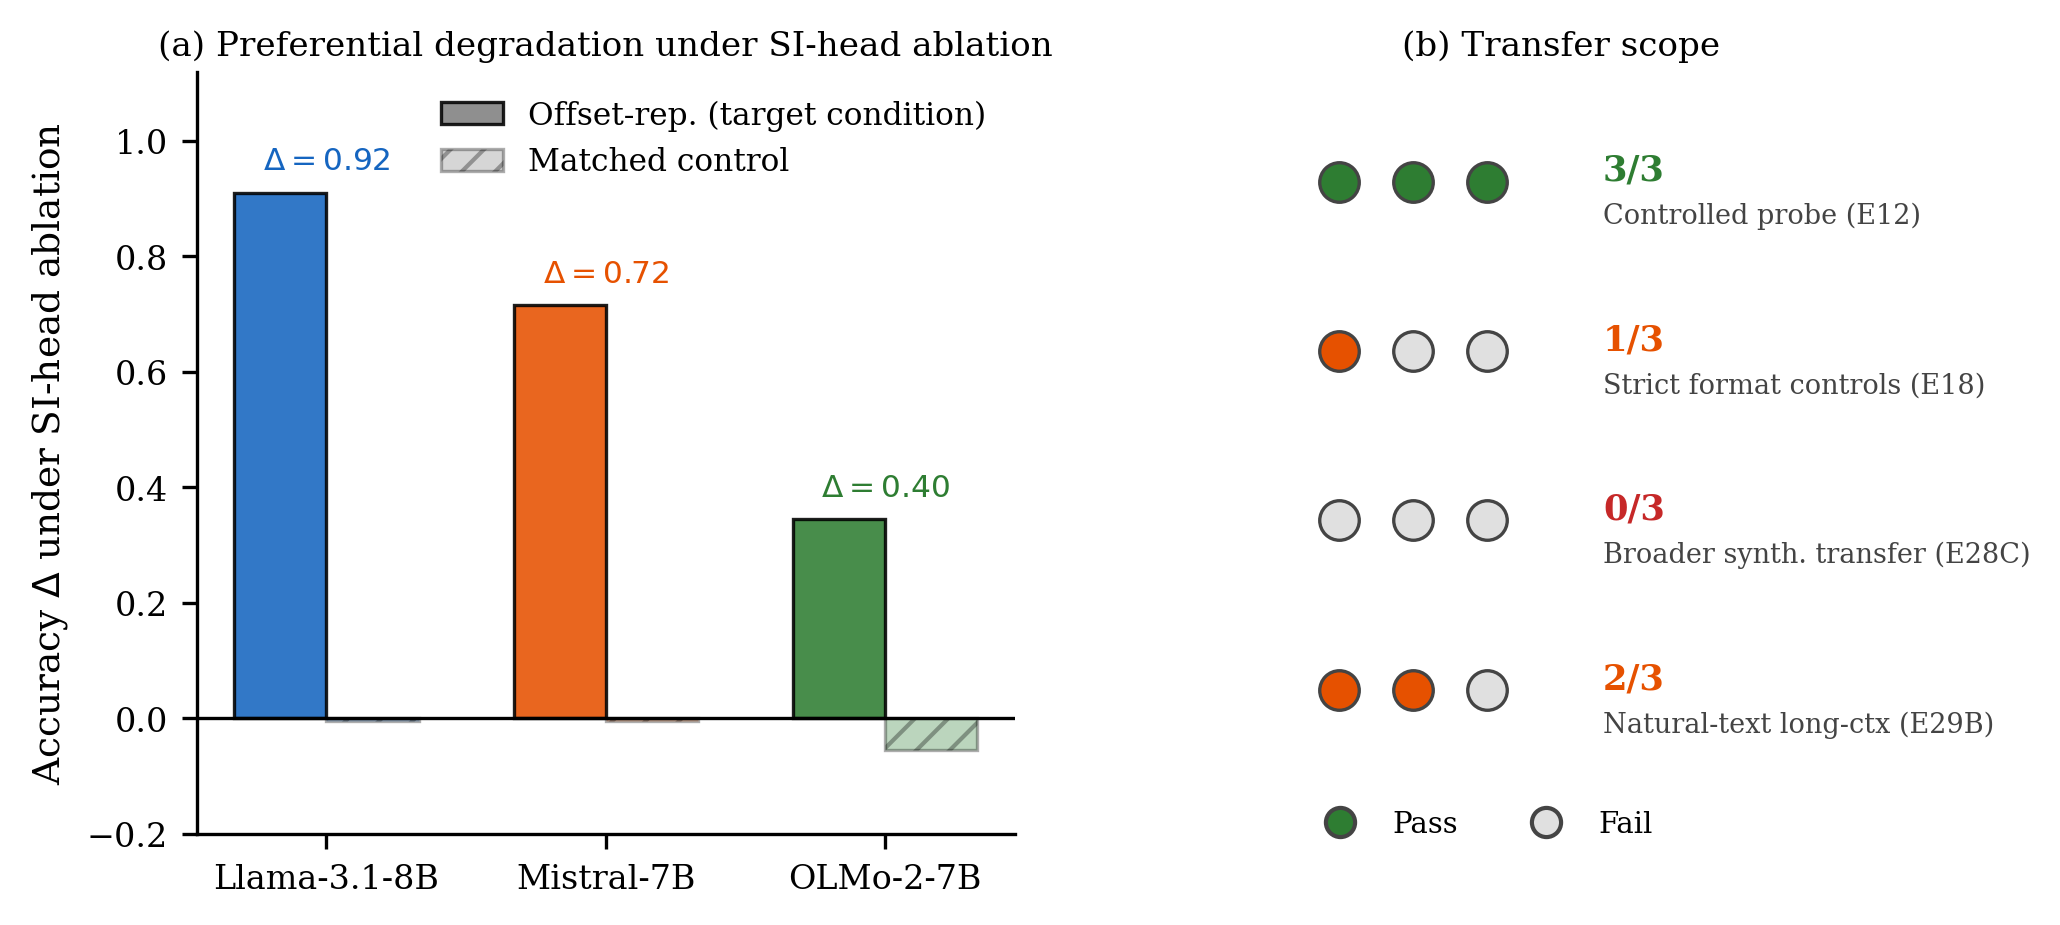
\includegraphics[width=0.84\textwidth]{../neurips2026/figures/fig_functional_sensitivity.png}
\caption{Functional sensitivity under SI-head ablation. \textbf{Left}: accuracy change under SI-head removal for offset-repetition (solid) vs.\ matched-control conditions (hatched); preferential gap ($\Delta$) is positive in all three models but decreases with SI amplitude (Llama $>$ Mistral $>$ OLMo). \textbf{Right}: transfer-scope summary across four probe settings; filled circles = model pass, empty = fail. Sensitivity is robust under the controlled probe (3/3) but narrows under stricter format controls (1/3) and broader synthetic families (0/3); natural-text long-context extension passes in Llama/Mistral (2/3).}
\label{fig:func_sensitivity}
\end{figure}

This result is therefore supportable as a bounded functional signal under intervention, not as a universal transfer law or a circuit-identity claim.

\section{Scope and Robustness Boundaries}

\paragraph{Functional boundary.}
The functional sensitivity result is strongest on the controlled offset-repetition probe and narrows under stricter and broader transfer settings: strict format controls are mixed, broader synthetic transfer is non-passing, and natural-text transfer is positive in Llama/Mistral but negative in OLMo.

\paragraph{Collective-ablation context.}
Ranked cumulative ablation robustly rejects linear depletion across tasks and models (0/18 linear BIC wins), showing non-linear accumulation of disruption under ordered head removal. However, matched non-SI controls show that this nonlinearity is not SI-unique (SI-ranked 0/9 linear vs.\ matched non-SI 1/9 linear; delta-BIC CI spans zero). We therefore treat this pattern as contextual organizational regularity, not as primary SI-specific mechanism evidence (Appendix~\ref{app:exp3p2}).

\paragraph{Integrated reading.}
These mixed secondary outcomes do not overturn the primary result; they bound its scope. They rule out broad claims of universal SI transfer and SI-unique collective organization, while leaving the strongest supported statement intact: head-level SI structure is intervention-sensitive in a specific, reproducible way. The main open alternatives concern \emph{where} this sensitivity transfers and \emph{which} training factors determine exploitation amplitude.

\paragraph{Open limitations.}
Cross-model causal attribution remains open because architecture, tokenizer, corpus, normalization, and optimization vary jointly; pretraining data volume and source are the most proximal candidate drivers given the Llama/Mistral vs.\ OLMo split, but this is untested. Specifically, we hypothesize that the density of code and formal mathematics in the pretraining corpus---domains governed by strict relative-offset rules such as syntax indentation and bracket matching---might exert the structural pressure necessary to develop high-capacity SI channels. This aligns with the stronger code emphasis in Llama and Mistral compared with OLMo's broader web-text mix. Llama/Mistral provide the strongest positive signal, OLMo is a weak-SI directional anchor, and the Qwen quickcheck does not directionally corroborate. The SI metric remains in-distribution and pair-weighted, and the theoretical lenses are framework-level rather than confirmed mechanisms. Finally, the seed-variance decomposition is proxy-scale (1.1B) and should not be read as a direct 7--8B seed-variance estimate. Full evidence-tier definitions, promotion rules, and control analyses are provided in Appendix~L.

\section{Discussion}

The evidence is best read as an organizing empirical frame, not an identified causal chain: RoPE provides SI capacity, training modulates exploitation amplitude, and intervention reveals structured SI usage. A notable anchor for this interpretation is that GPT-2 (absolute PE) still exhibits measurable SI structure, which supports a learned-computation reading rather than a RoPE-only artifact explanation. Within this frame, evidence strength is stratified rather than uniform.

\textbf{Established empirical findings.} The central contribution is a converging head-level specificity result: across all three primary models, SI-kernel intervention is load-bearing, and per-head disruption scales with SI amplitude under permutation-specificity, importance-matched, kernel-transplant, and local-bias controls. The head-level structure is strongest in Llama/Mistral and directionally present but compressed in OLMo. A broader 11-model consolidation shows that SI amplitude heterogeneity extends well beyond the primary trio. The functional sensitivity finding provides a supporting bound: controlled probe disruption is directionally consistent across models, with transfer scope limited to offset-structured retrieval contexts; a two-model (Llama, Mistral) naturalistic validation provides cross-architecture extension in the same direction. Cumulative ablation organization (Appendix~\ref{app:exp3p2}) is supporting context: collective nonlinearity is robust but not SI-unique.

\textbf{Interpretive framework.} We treat two primary lenses as complementary and provisional. The first is a \textit{frequency-domain lens} grounded in RoPE's structure. RoPE inner products decompose as a Fourier sum over offset: $Q_i \cdot R_{\theta}^{(i-j)} K_j = \sum_d [a_d \cos((i{-}j)\theta_d) + b_d \sin((i{-}j)\theta_d)]$. Shift-invariant heads are those where this expansion is approximately constant over offset---the offset-only component $g_h$ dominates. Importantly, the oscillatory structure of the learned kernel $g_h$ predicts disruption cost empirically: heads with higher DFT frequency content in their $g_h$ kernels (richer offset-specific routing patterns) show significantly larger disruption under SI-kernel subtraction (Spearman $\rho{=}0.437$, $p{=}2.2\times10^{-13}$, Llama; Appendix~B). This connects the theoretical framework directly to the intervention evidence, and explains why removing the SI kernel is not equivalent to a generic head perturbation. Representative kernels and spectra are shown in Appendix Figure~\ref{fig:kernels}. The second is \textit{Representational-Commitment Hypothesis (not an established mechanism)}: SI channels in current models appear stably allocated toward narrow positional/surface routing, with broader semantic SI usage under-realized. Two falsifiable predictions follow:
\begin{enumerate}
\item Continued pretraining with explicit SI-consistency pressure on semantic-invariance tasks should increase SI-linked functional disruption signatures on those tasks.
\item Short-horizon fine-tuning without such pretraining pressure should produce weaker or inconsistent retargeting of SI-linked functional signatures.
\end{enumerate}
A supplemental compressed-sensing-inspired lens is developed in Appendix~H. All three lenses are predictive frameworks rather than confirmed mechanisms.

\textbf{Actionable future test.} A concrete next step follows from both lenses: full-weight continued pretraining with explicit SI-consistency pressure on semantic invariance tasks. The prediction is that this should increase SI-linked disruption signatures on those tasks, while short-horizon fine-tuning should show weaker retargeting. Disconfirmation would be equally informative: if SI channels retarget quickly under short adaptation, or if pretraining-stage SI pressure does not shift SI-linked behavior, the commitment framing should be revised.

\section{Broader Impact}

Potential positive impact is methodological: the paper provides an auditable template for separating head-level specificity claims from collective-level and transfer-level claims, which can reduce over-interpretation in mechanistic interpretability studies. A second positive impact is practical hypothesis generation: if SI channels can be aligned to semantic invariances during pretraining, positional robustness and long-context retrieval may improve.

Potential negative impact is targeted degradation or steering of model behavior via structured logit-space interventions, especially if intervention recipes are over-generalized beyond their tested scope. We mitigate this by reporting non-supporting controls, separating primary from supporting evidence, and explicitly restricting claims to tested-model regularities.

\section{Conclusion}

This paper establishes a bounded empirical result: in three 7--8B RoPE models, SI structure is load-bearing under intervention, and head-level SI amplitude is a strong predictor of disruption cost under a converging control stack. The strongest positive evidence is concentrated in Llama and Mistral, with OLMo as a compressed directional anchor. A broader 11-model consolidation reinforces that SI amplitude heterogeneity is widespread rather than a single-pair anomaly.

What remains unresolved is equally clear. We do not identify causal drivers of the 6.5$\times$ cross-model SI-amplitude spread, do not provide matched-scale 7--8B RoPE-vs-NoPE causal training contrasts, and do not establish SI-unique collective organization or broad extra-family generalization. Functional probe sensitivity is model-conditional and probe-scoped; the naturalistic validation covers Llama and Mistral but not OLMo or non-RoPE architectures. Cumulative ablation organization is real but not SI-specific.

Why this matters is forward-looking: SI channels are present, load-bearing, and currently used unevenly across models. The representational-commitment and frequency-domain lenses provide a testable framework for pretraining design. The concrete prediction is that pretraining with explicit SI-consistency pressure on semantic invariance tasks should increase SI-linked functional signatures; short-horizon fine-tuning should show weaker retargeting. Validating or falsifying that prediction is the key next step, and the GPT-2 finding---that SI structure is learned even under absolute PE---suggests this pressure would find a receptive substrate even in architectures without RoPE's geometric prior.

\bibliographystyle{plainnat}
\bibliography{../neurips2026/references}
\appendix
\setcounter{figure}{0}
\setcounter{table}{0}
\renewcommand{\thefigure}{A\arabic{figure}}
\renewcommand{\thetable}{A\arabic{table}}
\renewcommand{\theHfigure}{appendix.figure.\arabic{figure}}
\renewcommand{\theHtable}{appendix.table.\arabic{table}}

\textit{This document is the supplementary material accompanying the main submission.
It provides full experimental details, extended results, and robustness analyses for the
main claims in the paper. References using Arabic numbering refer to the main paper;
appendix sections are lettered and can be read independently.}

\section*{Appendix overview}

\begin{itemize}
\item \textbf{A--D}: Primary measurement, intervention, and functional analyses.
\item \textbf{E--I}: Secondary analyses for scope limits and alternative explanations.
\item \textbf{J--K}: Statistical methodology and compute resources.
\item \textbf{L}: Consolidated robustness and attribution controls.
\item \textbf{M}: Exploratory toy-model causal probe (future-work motivation only).
\end{itemize}

\begin{figure}[htbp]
\centering
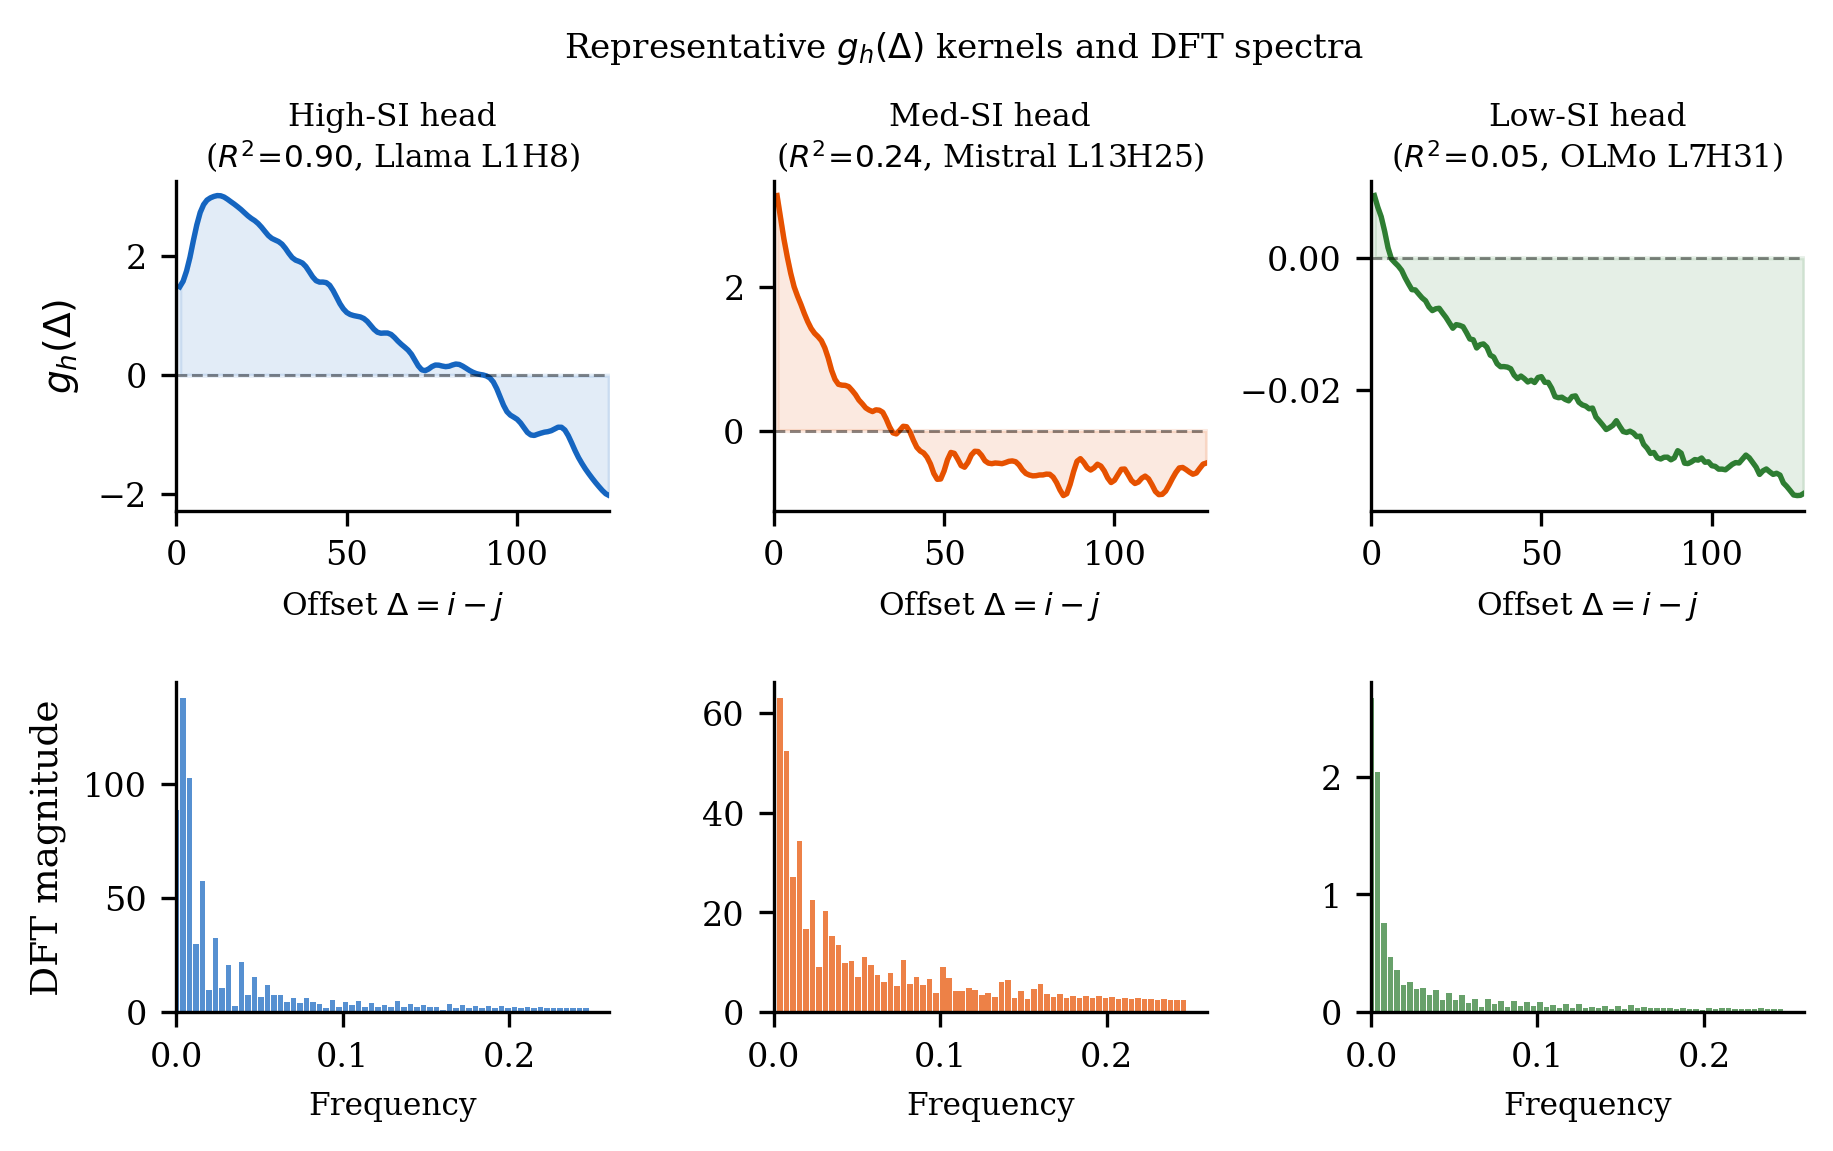
\includegraphics[width=\textwidth]{../neurips2026/figures/fig_kernel_examples.png}
\caption{Representative $g_h(\Delta)$ kernel shapes (top) and their DFT magnitude spectra (bottom) for high-, medium-, and low-SI heads. High-SI heads exhibit richer oscillatory structure with higher DFT energy, while low-SI heads are near-flat. This aligns with the main-text frequency-domain observation that higher DFT content predicts larger disruption under SI-kernel subtraction (Spearman $\rho{=}0.437$, $p{=}2.2\times10^{-13}$, Llama).}
\label{fig:kernels}
\end{figure}

\section{Experiment 1: Measurement of shift-invariant structure}
\label{app:exp1}

\subsection{Setup}

We measure the degree to which pre-softmax attention logits are approximated by a
head-specific shift-invariant function $g(\Delta)$ across a grid of 6 models $\times$ 3
datasets $\times$ 2 sequence lengths (36 combinations).

\paragraph{Models.} Llama-3.2-1B~\citep{dubey2024llama3} (RoPE + RMSNorm),
OLMo-1B~\citep{groeneveld2024olmo} (RoPE + LayerNorm),
TinyLlama-1.1B~\citep{zhang2024tinyllama} (RoPE + RMSNorm),
TinyLlama-NoPE-1.1B (no PE + RMSNorm, control),
GPT-2 small~\citep{radford2019language} (absolute PE + LayerNorm),
GPT-2 medium~\citep{radford2019language} (absolute PE + LayerNorm).

\paragraph{Datasets.} Wikipedia (wiki40b\_en\_pre2019), Python code (CodeSearchNet), and
synthetic random token sequences.

\paragraph{Sequence lengths.} 256 and 1024 tokens.

\paragraph{Measurement.} \textbf{Track A} fits $g(\Delta)$ directly to raw pre-softmax
logits via least-squares regression per head, reporting $R^2$ as the SI metric.
\textbf{Track B} uses a content-removed Gram matrix approach for cleaner positional signal
estimation. Preregistered threshold: early-layer (layers 0--1) pooled $R^2 > 0.80$ for
strong support; $0.40$--$0.80$ partial; $< 0.40$ falsification region.

\begin{table}[htbp]
\centering
\small
\caption{Main-text 7--8B SI-strength anchors (reported in Section~4; included here to reconcile appendix scale).}
\label{tab:appa_7b_r2_anchor}
\begin{tabular}{lc}
\toprule
Model & Mean per-head $R^2$ \\
\midrule
Llama-3.1-8B & 0.380 \\
Mistral-7B-v0.1 & 0.266 \\
OLMo-2-7B & 0.058 \\
\bottomrule
\end{tabular}
\end{table}

\begin{table}[htbp]
\centering
\small
\caption{7--8B per-head SI-strength distribution summary (same underlying head-level data used by Section~4 and RC10).}
\label{tab:appa_7b_r2_quantiles}
\begin{tabular}{lccccc}
\toprule
Model & Mean $R^2$ & Std & Q25 & Median & Q75 \\
\midrule
Llama-3.1-8B & 0.3803 & 0.1561 & 0.2545 & 0.3885 & 0.5040 \\
Mistral-7B-v0.1 & 0.2658 & 0.1430 & 0.1556 & 0.2401 & 0.3688 \\
OLMo-2-7B & 0.0576 & 0.0584 & 0.0153 & 0.0457 & 0.0814 \\
\bottomrule
\end{tabular}
\end{table}

\subsection{Detailed results}

\begin{figure}[htbp]
\centering
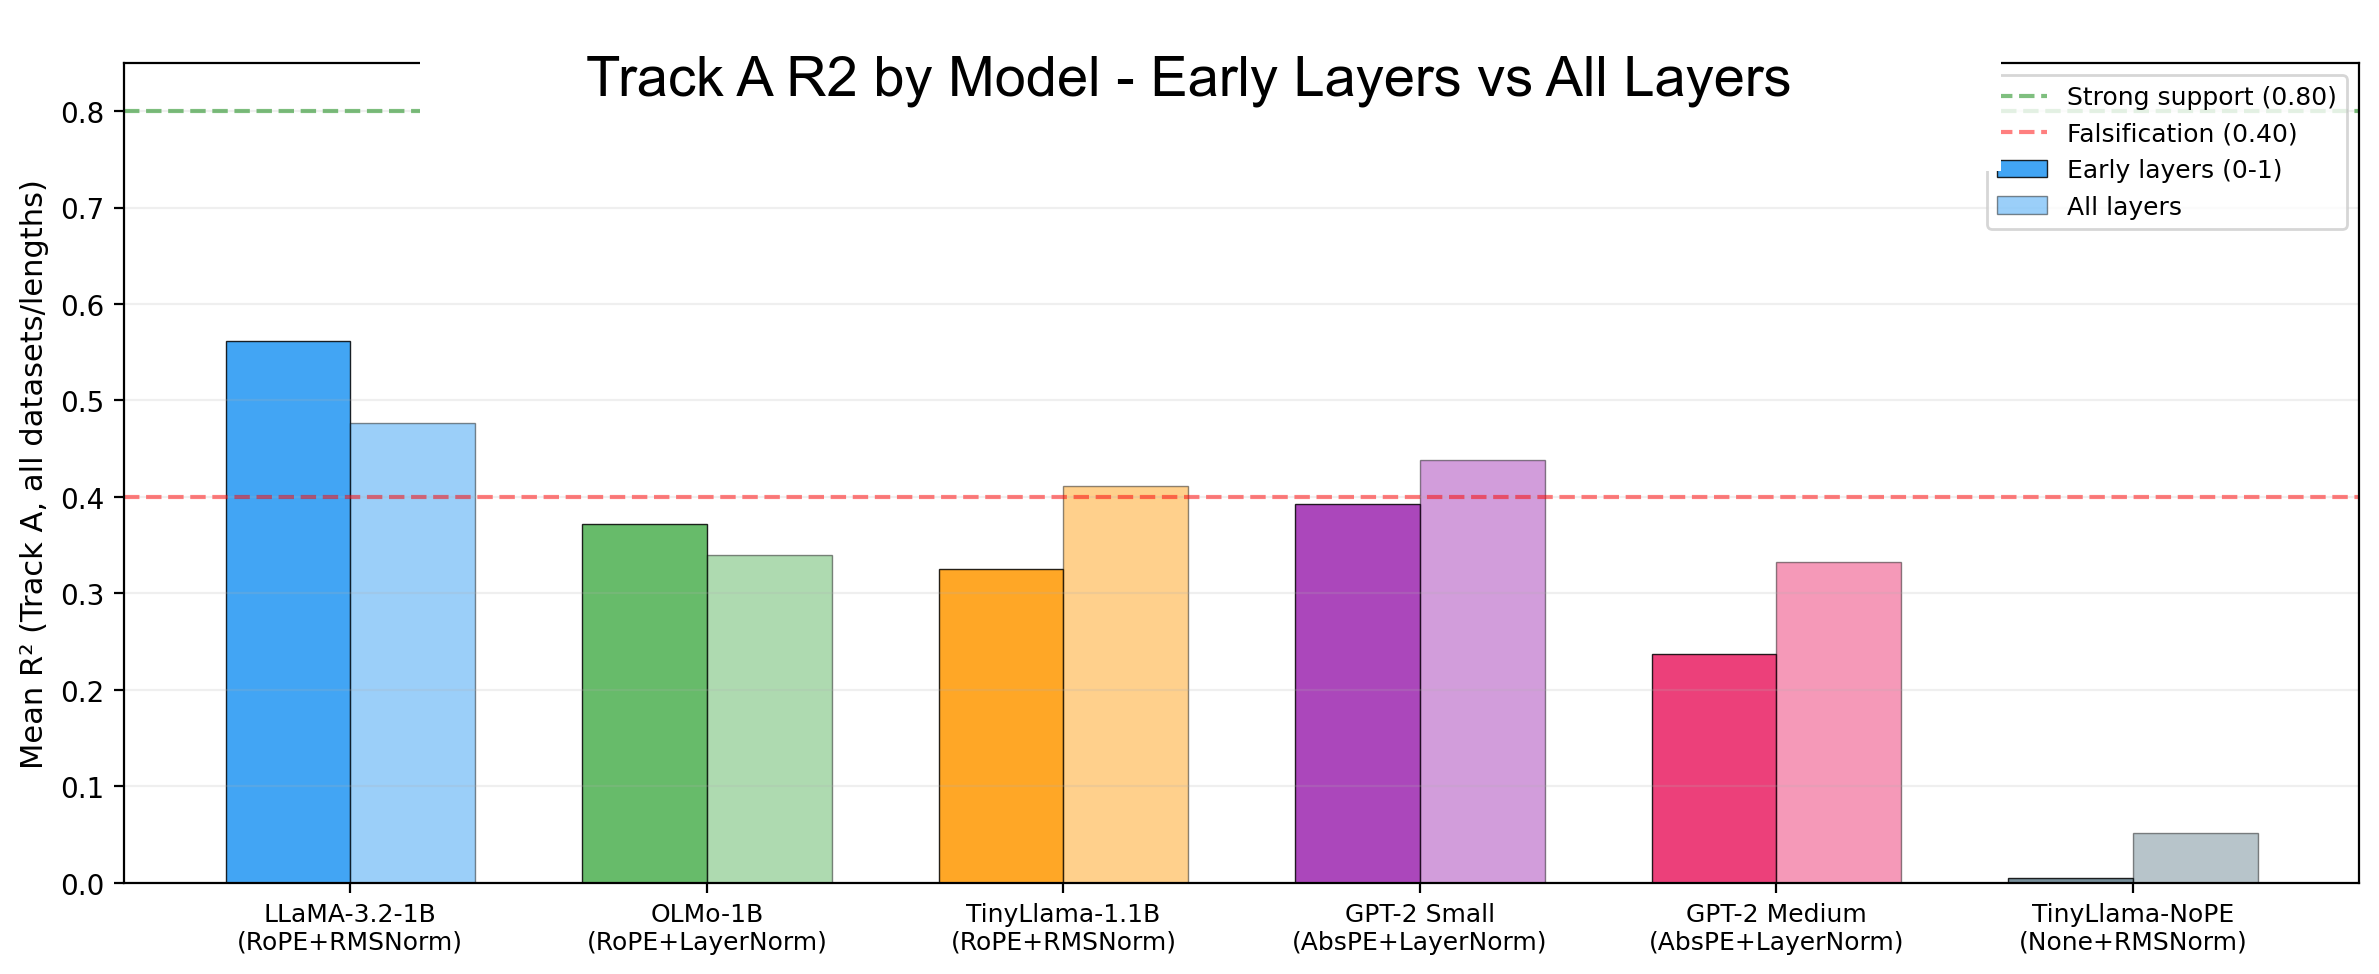
\includegraphics[width=0.95\textwidth]{../neurips2026/figures/fig2_r2_distributions.png}
\caption{Model-level Track-A SI summary across tested models (1B proxy scale; early layers vs.\ all layers). RoPE-equipped models are substantially above the TinyLlama-NoPE anchor in early layers, while GPT-2 anchors (absolute PE) remain non-trivial. This 1B proxy measurement motivates but does not replace the 7--8B primary-model heterogeneity reported in Section~4 and Figure~\ref{fig:setup_capacity}.}
\label{fig:r2_dist}
\end{figure}

\begin{table}[htbp]
    \caption{Track A early-layer $R^2$ by model, dataset, and sequence length (selected rows).}
    \centering
    \small
    \begin{tabular}{llccc}
        \toprule
        Model & Dataset & Len & Early $R^2$ & Overall $R^2$ \\
        \midrule
        Llama-3.2-1B & synthetic & 256 & 0.625 & 0.544 \\
        Llama-3.2-1B & synthetic & 1024 & 0.621 & 0.596 \\
        Llama-3.2-1B & wiki & 256 & 0.517 & 0.424 \\
        Llama-3.2-1B & wiki & 1024 & 0.523 & 0.414 \\
        OLMo-1B & synthetic & 256 & 0.453 & 0.388 \\
        OLMo-1B & wiki & 1024 & 0.346 & 0.300 \\
        TinyLlama-NoPE & synthetic & 256 & 0.008 & 0.023 \\
        TinyLlama-NoPE & wiki & 1024 & 0.002 & 0.074 \\
        \bottomrule
    \end{tabular}
\end{table}

\paragraph{Depth dependence.} All PE-equipped models show $R^2$ decay with depth.
TinyLlama shows an inverted early-layer pattern (lower early, higher overall), suggesting
some deeper heads develop specialized positional structure.

\paragraph{Dataset sensitivity.} Synthetic sequences yield the highest $R^2$ ($\sim$0.35
averaged across models), followed by Wikipedia ($\sim$0.30) and code ($\sim$0.30).

\paragraph{Track A vs Track B.} Track B centered diagnostics confirmed parity with CPU
baselines at machine epsilon across a 42-job centering granularity sweep.

\section{Experiment 2: Causal frequency interventions}
\label{app:exp2}

\subsection{Setup}

\paragraph{Hypotheses.} H1: High-frequency ablation hurts short-range more. H2:
Low-frequency ablation hurts long-range more.

\paragraph{Intervention.} Partition $D$ RoPE frequency pairs into high/low bands. Strong
ablation removes 60\% of targeted-band channels. Continuous attenuation at 25\%, 50\%, 75\%
severity rules out hard-zero artifacts. Norm-preserving rescaling (drift $\leq 0.05$).

\paragraph{Task suite.} Local copy-offset (short), local key-match (short), delayed copy
(long), long-range retrieval (long).

\paragraph{Models.} 1B: Llama-3.2-1B~\citep{dubey2024llama3},
OLMo-1B~\citep{groeneveld2024olmo}, TinyLlama-1.1B~\citep{zhang2024tinyllama}.
7--8B: Llama-3.1-8B~\citep{dubey2024llama3}, OLMo-2-7B~\citep{groeneveld2024olmo},
Mistral-7B~\citep{jiang2023mistral}.

\subsection{Detailed results}

\begin{table}[htbp]
    \caption{Complete Experiment 2 results across all analysis branches.}
    \centering
    \small
    \begin{tabular}{lcccc}
        \toprule
        Analysis & H1 effect & H1 status & H2 effect & H2 status \\
        \midrule
        1B confirmatory (3 models) & $+0.047$ & near-miss & $-0.155$ & reversed \\
        1B feasibility (Llama + OLMo) & $+0.097$ & pass & $-0.166$ & reversed \\
        7--8B Phase 2A (3 models) & $+0.112$ & pass & $-0.245$ & reversed \\
        Option D ablation (7--8B) & $+0.101$ & pass & $-0.205$ & reversed \\
        Option D attenuation 75\% & $+0.094$ & pass & $-0.195$ & reversed \\
        Option D attenuation 50\% & $+0.082$ & pass & $-0.182$ & reversed \\
        Option D attenuation 25\% & $+0.074$ & pass & $-0.132$ & reversed \\
        \bottomrule
    \end{tabular}
\end{table}

\paragraph{H2 interpretation.} The reversal is not an artifact of hard-zero ablation
(attenuation replicates), span overlap (fixed in Option D), or coarse averaging (pair-level
shows same direction). Low-frequency channels serve all dependency ranges.

\section{Experiment 3: Mechanistic theory battery}
\label{app:exp3}

\subsection{Setup}

Ten competing theories tested on Llama-3.1-8B~\citep{dubey2024llama3} and
OLMo-2-7B~\citep{groeneveld2024olmo}. High-SI heads defined as top quartile by per-head $R^2$.

\begin{table}[htbp]
    \caption{Full Experiment 3 theory battery results. Theories T2, T4, and T6 were not
    executed as part of the core Experiment 3 battery in this program; they appear as
    reserved entries in the theory numbering scheme.\textsuperscript{$\dagger$}}
    \centering
    \small
    \begin{tabular}{llccp{4.2cm}}
        \toprule
        Theory & Hypothesis & Llama & OLMo & Key metric \\
        \midrule
        T1 & SI $\leftrightarrow$ task perf. & \textcolor{red}{Not supp.} &
            \textcolor{red}{Not supp.} & $\Delta\text{drop} = -0.015$, $p > 0.97$ \\
        T3 & Cross-term corr. & Descriptive & Descriptive & $\rho$: $-0.11$ / $+0.05$ \\
        T5 & Subword continuation & \textcolor{red}{Not supp.} & \textcolor{red}{Not supp.}
            & Interaction reversed \\
        T5a & Boundary detection & \textcolor{blue}{Supported} & \textcolor{blue}{Supported}
            & All criteria met \\
        T7 & Induction feeders & \textcolor{blue}{Supported} & \textcolor{blue}{Supported}
            & High-SI feeds induction \\
        T7a & Activation patching & \textcolor{red}{Not supp.} & \textcolor{blue}{Supported}
            & $\rho = 0.06$ (NS) / $0.21$ \\
        T8 & Kernel ablation & \textcolor{blue}{Supported} & \textcolor{blue}{Supported}
            & Significant loss increase \\
        T9 & Freq-band feeders & Descriptive & Descriptive & $\rho_{\text{HF}} = 0.44$ / $0.21$ \\
        T10 & Feeder specificity & \textcolor{red}{Not supp.} & \textcolor{red}{Not supp.}
            & Not induction-specific \\
        \bottomrule
    \end{tabular}
\end{table}
\noindent\textsuperscript{$\dagger$}Only executed theories are reported in this table.

\paragraph{Note on T1 vs.\ T8.}
T1 failure (no per-head SI--task correlation; $p > 0.97$) is consistent with T8 support
(significant collective kernel ablation): when SI contributions are small and redundant
across heads, per-head SI--performance correlation is expected to be near zero even as
collective ablation cost is large.
T1 non-significance is therefore structurally predicted by the functional sensitivity finding (distributed
redundancy), not a contradiction of it.

\paragraph{T5a details.} Boundary detection criteria: (A) boundary attention $>$ chance,
(B) high-SI $>$ low-SI boundary attention, (C) effect survives content controls.
All three criteria met for Llama; A and C met for OLMo with B marginal.

\paragraph{T8 details.} Positional kernel $\hat{g}(\Delta)$ estimated per head via
least-squares, then subtracted from logits. Loss increase significant in both models.

\paragraph{T7/T10 interpretation boundary.}
T7 support means high-SI heads contribute to pathways that include induction heads.
T10 non-support means this feeder relationship is not induction-specific: high-SI heads
also feed non-induction targets. Accordingly, we use T7 as compatibility evidence for
ICL-relevant routing, but do not claim an induction-unique SI circuit identity.

\section{Experiment 3 Phase 2: Adjudication layer}
\label{app:exp3p2}

Eleven sub-experiments targeting unresolved mechanisms from the core battery.

\begin{table}[htbp]
    \caption{Phase 2 adjudication: full results across 11 sub-experiments.}
    \centering
    \small
    \begin{tabular}{llp{5.8cm}}
        \toprule
        Exp & Target & Key outcome \\
        \midrule
        A & Positional broadcast & Model-conditional: Llama specialized, OLMo uniform \\
        B & Boundary triviality & Non-trivial baseline signal; strict status model-conditional (Mistral clean, OLMo directional-null caveat, Llama gate-ambiguous) \\
        B-ext & Tokenizer feature audit & Llama expanded feature ablations block/reverse boundary signal, consistent with tokenizer-mediated routing \\
        C.1 & Redundancy model & Linear rejected in all 3-way cells (0/18 linear; 12/18 threshold, 6/18 logistic) \\
        C.2 & Superlinearity test & No superlinear support \\
        C.3 & Low-SI backup & Directional support for distributed backup \\
        D & Architecture tiebreaker & Weak unique-SI after prev-token control (Mistral) \\
        E & T5 vs T5a reconciliation & Boundary-primary resolution \\
        F & Proxy $R^2$ confound & Retained ($\Delta R^2 = 0.003$); underpowered \\
        G & Dose-response saturation & Mixed: OLMo early slope, Llama null \\
        H & Source/target spec & Mixed: Llama recovered specificity, OLMo null \\
        I & Tokenizer invariance & OLMo strict-pass ($0.75$); Llama strict-ambiguous (neither pass nor blocked) \\
        J & Conditional specialization & Interaction significant in both models; proxy-to-task sign transfer not yet stable \\
        K & Non-RoPE anchor & SI detected in GPT-2-medium and GPT-2-small; strict non-trivial boundary signal in both \\
        \bottomrule
    \end{tabular}
\end{table}

\paragraph{C.1: Redundancy-model details.} All three models (Llama, OLMo, Mistral) give zero BIC votes
to linear degradation in a 3-way comparison (threshold-piecewise, logistic-sigmoid, linear).
Per-model votes: 4/2/0 (threshold/logistic/linear), identical across all three; totals
are 12/18 threshold, 6/18 logistic, 0/18 linear.
Both non-linear models are consistent with the distributed-redundancy interpretation:
threshold-piecewise captures abrupt collapse; logistic-sigmoid captures smooth
accelerating collapse converging to the same collective-depletion structure.
This is the primary evidence for the distributed redundancy claim in the main paper.
The threshold finding is also directionally consistent with the phase-transition
prediction in Exp.~7B (see Appendix~H).

\paragraph{Gemma-2-9B fourth-family replication.}
The fourth-family replication executes on \texttt{google/gemma-2-9b} with the same cumulative-ablation fraction grid
$\{0,0.01,0.02,0.05,0.10,0.15,0.20,0.25,0.50\}$ and 5 seeds.
Per-head SI strength uses $n=500$ random-sequence evaluations (length 128; max offset 64).
Kernel-ablation LM loss uses 40 random sequences (length 128).
Cumulative-ablation curves use 40 key-match and 40 long-range retrieval prompts per seed,
plus LM-loss evaluations on up to 20 random sequences per fraction/seed.
Observed BIC votes are threshold in all 3 task cells (0/3 linear).

\subsection{Reinforcement analyses (R1--R8)}
\label{app:reinforcement}

\paragraph{Evidence window.}
This subsection summarizes reinforcement analyses finalized by April 28, 2026. These checks were designed to tighten claim scope, stress-test key conclusions, and separate robust findings from model-conditional or mixed outcomes.

\begin{table}[htbp]
    \caption{Reinforcement analyses: prespecified criteria, outcomes, and claim impact.}
    \centering
    \small
    \begin{tabular}{p{0.8cm}p{2.3cm}p{2.5cm}p{2.7cm}p{2.9cm}}
        \toprule
        ID & Analysis & Prespecified criterion & Outcome & Claim impact \\
        \midrule
        R1 &
        Multidomain strict-gate adjudication &
        Stable blocked or stable clean under pooled multidomain rule &
        Ambiguous overall (wiki ambiguous, code stable-clean, dialogue ambiguous); neither aggregate gate passes &
        Keep Llama strict status as ambiguous; avoid strict blocked/strict clean claim \\

        R2 &
        Dependence-aware sensitivity reanalysis &
        Direction consistency under sequence-cluster sensitivity checks &
        7/8 directional checks supported; unsupported cell is OLMo boundary non-triviality &
        Main narrative retained with explicit OLMo boundary caveat \\

        R3 &
        Core-battery replication &
        Completion of T8 (kernel ablation), T5a (boundary detection), Phase-2 C.1/C.2, and interaction checks &
        Positive overall replication (kernel load-bearing, strict-B clean, C1 threshold-supported) &
        Upgrades prior pending status to three-model core-battery support with attribution caveat \\

        R4 &
        PE-scheme comparison &
        Non-RoPE anchors should show SI structure with non-trivial boundary signal &
        Positive in both GPT-2 anchors (2/2 replications) &
        Narrows RoPE-only confound \\

        R5 &
        Task-grounded transfer check &
        Significant interaction and sign-concordance $\geq 3/4$ per model &
        Interaction significant in both models, but sign transfer fails (Llama 1/4, OLMo 2/4) &
        Keep interaction-level claim; downgrade regime semantics to proxy-specific \\

        R2a &
        OLMo boundary-power reinforcement &
        Domain-level practical-positive support for boundary non-triviality &
        Stable-clean statuses appear by domain, but directional support fails in all domains (0/3) &
        Reinforces conservative OLMo boundary caveat \\

        R5a &
        Regime-alignment reinforcement &
        Significant interaction plus sign-concordance threshold in mapped regimes &
        Interaction remains significant; transfer still fails (Llama 1/2, OLMo 1/2) &
        Confirms interaction-level signal; regime semantics remain proxy-specific \\

        R6 &
        Random-order ablation control &
        Threshold preference should survive non-ranked removal order &
        Strong replication (Llama 7/10, Mistral 9/10, OLMo 10/10; 26/30 threshold-majority) &
        Strengthens collective ablation robustness against ranking-order artifacts \\

        R7 &
        Kernel-permutation specificity &
        True SI-kernel perturbation should exceed offset-permuted perturbation &
        Supported in all primary models (Llama 3.2774, Mistral 3.1926, OLMo 0.0427; one-sided bootstrap $p=2.0\times10^{-4}$ each) &
        Strengthens perturbation-specific mechanism interpretation \\

        R8 &
        High-SI head-identity stability &
        Cross-domain overlap should exceed random expectation &
        Partial stability in both models (Llama 3-way Jaccard 0.594, OLMo 0.427; both above random) &
        Supports head-set reuse with caveat (not high-confidence stable) \\
        \bottomrule
    \end{tabular}
\end{table}

\paragraph{Reinforcement summary.}
The reinforcement checks are consistent with the main-paper framing: kernel-level specificity and ranked-ablation robustness replicate, strict multidomain adjudication remains mixed, and transfer-direction claims remain model-conditional.

\paragraph{Functional sensitivity probe protocol.}
E12 evaluates three primary models on 200 prompts per condition (offset-repetition and matched control), reporting both accuracy and target-token log-probability under intact vs.\ high-SI-head ablation. Model-level support is assigned by preferential-degradation direction on valid metrics.

\section{Experiment 4: SI-guided fine-tuning}
\label{app:exp4}

\subsection{Setup}

Tests whether SI structure can be strategically leveraged during fine-tuning for mathematical
reasoning. Three sub-experiments in gated progression.

\paragraph{Models.} Llama-3.1-8B~\citep{dubey2024llama3} and
OLMo-2-7B~\citep{groeneveld2024olmo} for both 4A and 4C.

\paragraph{Training.} QLoRA with attention/MLP adapter injection, 250--300 steps, batch
size 1, learning rate $2 \times 10^{-4}$. Math training mix: digit arithmetic, counting
chains, modular arithmetic, sequence continuation (120 examples/task) + 20\% wiki/instruction
control.

\paragraph{Evaluation.} Math accuracy is measured as 4-shot accuracy on a 200-example
subset of the MATH benchmark~\citep{hendrycks2021math}, drawn from the \emph{Number Theory}
and \emph{Counting \& Probability} categories. These categories were selected for their
alignment with the training mix (arithmetic and combinatorial reasoning). Results may not
generalize to harder MATH categories (Algebra Level 4--5, Geometry, Precalculus). The
observed 59--66\% accuracy range reflects the relatively accessible nature of this subset.

\paragraph{SI head definition.} Top quartile by per-head $R^2$ from Experiment 3 Phase 2.

\subsection{Results}

\paragraph{4C: SI trajectory under fine-tuning (Llama-3.1-8B and OLMo-2-7B).} Snapshots at
steps 0, 50, 100, 150, 200, 250, 300 show minimal drift in both models: Llama mean
$\Delta R^2 = +0.0019$, boundary-$d$ change $= -0.016$; OLMo mean $\Delta R^2 = -0.0010$,
boundary-$d$ change $= -0.012$. Head-rank ordering is preserved throughout. SI structure
is stable in the short-to-medium fine-tuning regime; behavior under extended fine-tuning
(thousands of steps) remains untested.

\paragraph{4A: SI-aware LoRA comparison (cross-model).} 30 runs
(5 conditions $\times$ 3 seeds $\times$ 2 models):

\begin{table}[htbp]
    \caption{Exp.~4A results: all SI-routing conditions vs.\ baseline, by model.}
    \centering
    \small
    \begin{tabular}{lllcc}
        \toprule
        Model & Comparison & Accuracy $\Delta$ & 95\% CI & $p$ \\
        \midrule
        Llama-3.1-8B & (a) SI-protecting vs (b) uniform & $-0.011$ & $[-0.057, +0.034]$ & $0.668$ \\
        OLMo-2-7B & (a) SI-protecting vs (b) uniform & $-0.009$ & $[-0.025, +0.006]$ & $0.355$ \\
        Llama-3.1-8B & (e) SI-amplified vs (d) baseline & $-0.015$ & $[-0.049, +0.019]$ & $0.489$ \\
        OLMo-2-7B & (e) SI-amplified vs (d) baseline & $-0.003$ & $[-0.019, +0.013]$ & $0.742$ \\
        Llama-3.1-8B & (b) uniform vs (d) baseline & $-0.021$ & $[-0.060, +0.018]$ & $0.405$ \\
        OLMo-2-7B & (b) uniform vs (d) baseline & $+0.004$ & $[-0.014, +0.022]$ & $0.691$ \\
        \bottomrule
    \end{tabular}
\end{table}

All conditions are null in both models (Llama means: 0.864--0.887; OLMo means: 0.630--0.647).
4B (SI-loss-augmented training) deferred pending 4A signal.

\section{Experiment 5: Tokenizer effect audit}
\label{app:exp5}

\subsection{Setup}

Four sub-experiments auditing tokenizer dependence and boundary-linked SI behavior.
These analyses are model-conditional diagnostics, not a full causal decomposition of
cross-model SI-strength heterogeneity.

\paragraph{5A.} 6 models across 4 tokenizer families (GPT-2, Llama, OLMo, Pythia).

\paragraph{5B.} Llama-2-7B~\citep{touvron2023llama2} vs.\ Llama-3.1-8B~\citep{dubey2024llama3}:
same architecture family, different tokenizer (32k BPE vs.\ 128k BPE). Note that these
models also differ in training data, scale, and RLHF; 5B provides correlational evidence,
with strict causal attribution depending on 5C.

\paragraph{5C.} 12 perturbation cells $\times$ 2 models: fake boundaries, character
decomposition, morpheme breaks, boundary merges, random resegmentation.

\paragraph{5D.} 5 domains: wiki (baseline), code, dialogue, technical, adversarial BPE.

\subsection{Results}

\paragraph{5B: Head identity shuffles with tokenizer.} Top-quartile SI head overlap between
Llama-2 and Llama-3.1: Jaccard $J = 0.177$ (17.7\% shared). Rank correlation $\rho = 0.048$
(non-significant). Changing the tokenizer while holding architecture family constant
substantially reassigns which heads develop SI structure; note the confound with other
model differences (see Setup above).

\paragraph{5C: Causal perturbation results.} Tests run on 12 perturbation cells $\times$ 2
models (Llama-3.1-8B and OLMo-2-7B), evaluating mean SI head attention weight at boundary
vs.\ continuation positions across $n \approx 512 \times 24 = 12{,}288$ position-pairs per
model (24 sequences $\times$ 512 positions). The large $n$ explains the extreme $p$-values; the
effect sizes ($\Delta \approx +0.017$) are small in absolute terms. No correction for the
12-cell family is reported.
\begin{table}[htbp]
    \caption{Exp.~5C perturbation effects on SI attention.}
    \centering
    \small
    \begin{tabular}{lccc}
        \toprule
        Perturbation & Llama $\Delta$ attention & $p$ & OLMo effect \\
        \midrule
        Fake boundary insertion + prefix & $+0.017$ to $+0.052$ & $< 10^{-21}$ & Large \\
        Character decomposition & $+0.015$ to $+0.017$ & $< 10^{-34}$ & Large \\
        Random resegmentation & $+0.003$ to $+0.005$ & $> 0.05$ & Null \\
        \bottomrule
    \end{tabular}
\end{table}

These perturbations support tokenizer mediation of boundary-linked SI behavior in the
tested model configurations, but do not identify tokenizer vocabulary overlap as the
driver of cross-model SI amplitude differences. Note that the extraordinarily small
$p$-values reflect the large $n$, not large effect sizes; the practical effect
($\Delta \approx 0.017$) should be interpreted in context.

\paragraph{5D: Domain robustness.} Llama: dialogue $+0.057\, R^2$; technical $-0.040\, R^2$.
OLMo: dialogue $+0.027$; technical $-0.004$ (more stable). SI is domain-general infrastructure
with $\pm 0.06$ variation across very different text types including adversarial BPE sequences.

\paragraph{5A: Cross-family.} SI present in all 4 tokenizer families. Pythia anomaly: NaN
boundary dependence indices despite 80--99\% classifier accuracy; 4/6 models have finite
boundary measurements.

\section{Experiment 6: SI-guided knowledge localization}
\label{app:exp6}

\subsection{Setup}

Two completed intervention strategies test whether localizing math computation to SI channels
improves reasoning performance in the finalized evidence set:
\begin{enumerate}
\item 6A: Gradient routing (math gradients exclusively through SI head parameters)
\item 6B: Anti-localization loss (penalize attention localization in non-SI heads)
\end{enumerate}

Models: Llama-3.1-8B~\citep{dubey2024llama3} and TinyLlama-1.1B~\citep{zhang2024tinyllama}
(6A, 6B, 6C); OLMo-2-7B~\citep{groeneveld2024olmo} (6A). 3 seeds per model per condition.
Evaluation: math accuracy (4-shot), wiki perplexity.

\subsection{Results}

\paragraph{6A: Gradient routing.}
\begin{table}[htbp]
    \caption{Exp.~6A gradient routing results.}
    \centering
    \small
    \begin{tabular}{lccccc}
        \toprule
        Model & Math $\Delta$ (pp) & $p$ & PPL $\Delta$ & $p$ & Interpretation \\
        \midrule
        Llama-3.1-8B & $-12.3$ & $0.012$ & $-0.535$ & $0.003$ & SI disruption at scale \\
        TinyLlama-1.1B & $-0.2$ & $0.881$ & $-1.227$ & $0.003$ & Scale-dependent \\
        \bottomrule
    \end{tabular}
\end{table}

At 8B scale, math accuracy is significantly harmed while language modeling improves. The
scale asymmetry reflects that larger models have optimized SI allocations that routing disrupts.

\paragraph{6B: Anti-localization.} TinyLlama: math $\Delta = -0.5$ pp ($p = 0.65$, null).
Llama-3.1-8B seed 0: math $\Delta = -4.4$ pp (directional, partial data).

\paragraph{Submission scope note.}
Main-paper claims use only completed 6A/6B outcomes. Within completed sub-experiments, no
positive math-accuracy gain is observed.

\paragraph{Combined interpretation.} Among the completed sub-experiments
(6A: gradient routing; 6B: anti-localization), both are null or harmful.
This supports a conservative, scope-limited conclusion:
``every completed Experiment 6 sub-experiment is null or harmful in the tested settings.''
Combined with Exp.~4's null LoRA routing and immutability results across two model
families, the available evidence suggests SI is difficult to productively redirect
with post-hoc routing constraints in the evaluated regime.

\section{Experiment 7: CS-inspired framework validation}
\label{app:exp7}

\subsection{Setup}

\paragraph{7A: Welch-gap proxy relation (audited).} For each model and sequence length, we
compute analytic proxy coherence descriptors from PE metadata (PE type, head dimension, and
RoPE $\theta$ schedule), then join these descriptors with Track-A mean $\bar{R}^2$. Because
coherence descriptors are repeated across dataset rows, the primary analysis is model-level
($n=6$ unique models). The 36-row table (6 models $\times$ 2 sequence lengths $\times$ 3
datasets) is retained only as exploratory pseudo-replicated context.

\paragraph{7B: Phase-transition analogue.} Models: Llama-3.1-8B~\citep{dubey2024llama3}
and OLMo-2-7B~\citep{groeneveld2024olmo}. Sequence lengths: 256, 512, 1024. Protocol:
progressively ablate SI heads ranked by $R^2$, evaluate at each fraction
(0, 5, 10, 15, 20, 25, 35, 50, 75\% ablated), 3 seeds $\times$ 128 sequences per seed.
Compute observed critical point as inflection of degradation curve. Compare to
$m^* = C \cdot s_{\text{eff}} \cdot \log(N / s_{\text{eff}})$ where $s_{\text{eff}} = N \cdot \bar{b}$.
In the corrected canonical run, $C$ uses single-condition calibration on
Llama-3.1-8B at sequence length 256 ($C=7.057$), with 5 remaining conditions
reported out-of-sample. A global-fit reference ($C=7.834$) is reported separately.

\subsection{Results}

\paragraph{7A: Coherence-gap proxy relation is mixed at model level.}

\begin{table}[htbp]
    \caption{Exp.~7A: coherence gap vs.\ $\bar{R}^2$ correlation results.}
    \centering
    \small
    \begin{tabular}{lccc}
        \toprule
        Metric & Value & Notes & $p$ \\
        \midrule
        Pearson $r$ (model-level) & $+0.731$ & $n=6$ models & $0.099$ \\
        Spearman $\rho$ (model-level) & $+0.516$ & $n=6$ models & $0.295$ \\
        Permutation (two-sided, model-level) & $0.141$ & exact shuffles & --- \\
        Pearson $r$ (36-row exploratory) & $+0.609$ & pseudo-replicated rows & $8.1\times10^{-5}$ \\
        \bottomrule
    \end{tabular}
\end{table}

This is a proxy-scale, model-level analysis. The model-level relation is directionally
positive but not statistically decisive, and the 36-row correlation is exploratory because
coherence features repeat by model/length. We therefore treat 7A as suggestive
framework evidence rather than confirmatory mechanism evidence.

\paragraph{Expanded coherence-gap proxy panel (11 models).}
An expanded coherence refresh over an 11-model breadth panel (Appendix~L) is mixed:
Pearson $r=0.577$ (two-sided $p=0.063$), Spearman $\rho=0.500$ ($p=0.117$), and
permutation two-sided $p=0.070$. Direction is consistent with 7A, but significance is
non-decisive at this panel size. We therefore treat the coherence-gap lens as
framework-level rather than established mechanism evidence at current scale.

\paragraph{7B: Phase-transition critical point.}

Using canonical single-condition calibration ($C=7.057$ on Llama-3.1-8B, length 256),
Pearson $r=-0.959$ ($p=0.0025$) and Spearman $\rho=-0.878$ ($p=0.021$) between predicted
and observed thresholds across 6 conditions. Out-of-sample (excluding the calibrated
condition), Pearson remains strong ($r=-0.986$, $p=0.0019$) while Spearman is directional
but marginal ($\rho=-0.866$, $p=0.058$, $n=5$). BIC model comparison remains threshold-piecewise
preferred in 6/6 cases (consistent with Phase-2 sub-experiment C.1 unanimous preference). This remains
preliminary evidence ($n=6$ conditions, effective $n \approx 2$ independent model families
due to sequence-length correlation within models) requiring replication across additional
distinct model families.

\section{Experiment 8: Tokenizer analysis via SI structure}
\label{app:exp8}

\subsection{Setup}

\paragraph{8A: Boundary discrimination metrics.} Models: GPT-2-small~\citep{radford2019language},
TinyLlama-1.1B~\citep{zhang2024tinyllama}, Llama-3.1-8B~\citep{dubey2024llama3},
OLMo-2-7B~\citep{groeneveld2024olmo}. 24 sequences of length 512 (Wikipedia). Boundary
definition: position $t$ is a word boundary iff $\text{word\_id}[t] \ne \text{word\_id}[t-1]$
(using tokenizer fast API word IDs). Three metrics per model:
\begin{itemize}
    \item \textbf{BDI}: mean $A_h(t, t{-}1)$ at boundary minus at continuation positions.
    \item \textbf{BAC}: $\text{BDI}_\text{SI} / \text{BDI}_\text{non-SI}$.
    \item \textbf{KOA}: fraction of $\{d_{b_j} - d_{b_{j-1}}\}$ that are multiples of
        head's dominant kernel offset $\Delta^* = \arg\max_\Delta \hat{g}(\Delta)$.
\end{itemize}

Preregistered hypotheses: H1: $\text{BDI}_\text{SI} > 0$; H2: $\text{BDI}_\text{SI} >
\text{BDI}_\text{non-SI}$; H3: $\text{BAC} > 1$; H4: $\text{KOA} > $ chance.

\paragraph{8B: Tokenizer-aware pruning.} Models: Llama-3.1-8B~\citep{dubey2024llama3} and
OLMo-2-7B~\citep{groeneveld2024olmo}. Five mask types $\times$ 9 ablation fractions
(0, 5, 10, 15, 20, 25, 35, 50, 75\% ablated). Mask types: (1) si\_matched: remove
lowest-$R^2$ heads per model's own tokenizer; (2) si\_mismatched: use cross-model SI
ranking (Llama mask applied to OLMo, vice versa); (3) entropy: remove lowest-entropy heads;
(4) activation: remove lowest-activation-norm heads; (5) random: matched-cardinality random
removal. Evaluation: 4-shot math accuracy (MATH subset) and wiki perplexity. Area under
degradation curve (AUDC) and paired $t$-tests across fraction levels.

\subsection{Results: 8A}

Primary BDI/BAC/KOA runs are complete on small models (GPT-2-small and TinyLlama-1.1B).
7--8B BDI/BAC/KOA results are treated as non-primary in this submission snapshot and
are not used for preregistered 8A claim adjudication.
An exploratory all-model SIBAS variant was run separately and is not used for the
preregistered BDI/BAC/KOA claims reported here.

\begin{table}[htbp]
    \caption{8A boundary discrimination full results (small models only; 7--8B-scale pending).}
    \centering
    \small
    \begin{tabular}{lccccc}
        \toprule
        Model & BDI$_\text{SI}$ & $p$(H1) & $\Delta$BDI & $p$(H2) & Cohen's $d$ \\
        \midrule
        GPT-2-small & $+0.026$ & $1.3\times10^{-15}$ & $+0.026$ & $6.2\times10^{-15}$ & $5.14$ \\
        TinyLlama-1.1B & $+0.008$ & $4.1\times10^{-12}$ & $+0.010$ & $1.1\times10^{-13}$ & $4.58$ \\
        \bottomrule
    \end{tabular}
\end{table}

H3 (BAC$>$1) is not supported as preregistered: BAC is negative because non-SI BDI is
slightly negative. The unexpected negative BAC is a secondary observation requiring
follow-up; it is not a stronger version of the preregistered hypothesis.

H4 (KOA$>$chance) requires validation against a proper null distribution (random boundary
spacings or low-SI heads). KOA values near 1.0 for both models require this calibration
before H4 is interpretable. BDI$\times R^2$ Spearman $\rho = 0.407$ (GPT-2, $p < 0.001$)
and $0.329$ (TinyLlama, $p < 0.001$) confirm boundary discrimination as continuous in SI degree.

\subsection{Results: 8B}

\begin{table}[htbp]
    \caption{8B tokenizer-aware pruning on Llama-3.1-8B: early-ablation comparison.}
    \centering
    \small
    \begin{tabular}{lccc}
        \toprule
        Fraction ablated & si\_matched math & si\_mismatched math & Gap (pp) \\
        \midrule
        5\% & 0.662 & 0.369 & $+29.3$ \\
        10\% & 0.731 & 0.369 & $+36.2$ \\
        15\% & 0.562 & 0.212 & $+35.0$ \\
        \bottomrule
    \end{tabular}
\end{table}

The pre-specified primary comparison is SI-matched vs.\ SI-mismatched ($\alpha = 0.05$,
no correction): $p = 0.034$ on Llama-3.1-8B. Exploratory comparisons: matched vs.\ entropy
$p = 0.003$; matched vs.\ activation $p = 0.017$; matched vs.\ random $p = 0.337$ (ns). The paired
$t$-test treats ablation fractions as independent paired observations, which may not fully
account for serial correlation in the degradation trajectory; AUDC is the primary summary
statistic and $t$-tests are secondary.

OLMo-2-7B shows reversed ordering (mismatched outperforms matched at all fractions,
0--35\% ablation range). We attribute this to OLMo's weak SI signal (mean $R^2 = 0.058$
vs.\ Llama's $0.380$): with noisy SI classification, the top-quartile SI heads are not
reliably the most important for tokenizer-driven processing. SI-matched pruning should
therefore be treated as a model-conditional tool.

\begin{table}[htbp]
    \caption{8B primary matched-vs-mismatched comparison by model (AUDC summary).}
    \centering
    \small
    \begin{tabular}{lcccc}
        \toprule
        Model & Matched math AUDC & Mismatched math AUDC & Mean diff & $p$ \\
        \midrule
        Llama-3.1-8B & 0.261 & 0.198 & $+0.137$ & 0.034 \\
        OLMo-2-7B & 0.168 & 0.251 & $-0.160$ & 0.015 \\
        \bottomrule
    \end{tabular}
\end{table}

\section{Statistical methodology}
\label{app:stats}

All confirmatory tests use Holm-corrected $p$-values within each hypothesis family.
Bootstrap confidence intervals (10,000 resamples or 2,000 for Exp.~7A) for effect size
estimation. Stouffer meta-analysis combines evidence across models. Exploratory analyses
are clearly demarcated and non-retroactive to confirmatory labels. Preregistered hypothesis
families are locked before execution with explicit confirmatory/exploratory split. The
BDI, BAC, and KOA hypotheses (Exp.~8A) were preregistered before small-model execution.
In main-text reporting, we standardize summary order as effect size $\rightarrow$ confidence interval $\rightarrow$ $p$-value (when reported), and we include practical-magnitude interpretation alongside significance tests.

\paragraph{Preregistration and reproducibility materials.}
Preregistration documents, analysis scripts, and reproduction instructions are provided in the anonymous supplementary package. We use this package as the canonical source during review; a persistent external archive will be released at camera-ready.

\section{Compute resources}
\label{app:compute}

Experiments conducted on NVIDIA A100 (40GB) and A100/H100 (80GB) GPUs. Approximate
GPU-hours per experiment: Exp.~1: 24; Exp.~2: 48; Exp.~3 core: 48; Exp.~3 Phase 2: 40;
Exp.~4: 16; Exp.~5: 24; Exp.~6: 12 (partial); Exp.~7A: $<$1; Exp.~7B: 18; Exp.~8A: 4;
Exp.~8B: 24. Total: $\sim$260 GPU-hours reported; additional compute for preliminary and
failed runs not included. Exp.~8B on OLMo required a 48GB GPU (A6000) due to OOM on 16GB
cards during multi-fraction evaluation.

\section{Completed Robustness and Attribution Controls}
\label{app:running}

\begin{table}[htbp]
\centering
\small
\caption{Evidence provenance map for headline claims (addresses 1B vs.\ 7--8B sourcing). All headline claims use 7--8B primary models; 1B models serve as scope anchors and proxy controls only.}
\label{tab:provenance_map}
\begin{tabular}{p{3.6cm}p{2.9cm}p{4.4cm}}
\toprule
Headline claim & Primary scale & Provenance in this paper \\
\midrule
SI-strength heterogeneity (0.380/0.266/0.058) and kernel-subtraction load-bearing deltas (Appendix D, T8) & 7--8B & Main text Sections 4--5; 7--8B primary models \\
Breadth heterogeneity extension (11-model panel; max/min mean-$R^2$ ratio $140\times$) & Mixed-scale breadth panel & Appendix~L (descriptive breadth consolidation; non-promotional for causal attribution) \\
NoPE anchor (early-layer $R^2<0.01$) & 1.1B control & Main text scope anchor; detailed measurement tables in Appendix A \\
Checkpoint trajectory consistency (Appendix D, E4) & 7B (OLMo only) & Main-text scope/consistency note; not promoted as cross-model dynamics proof \\
Linear rejection (0/18, 26/30, 0/6) + Gemma directional replication (0/3) & 7--8B (+simplified Gemma protocol) & Appendix-first contextual ablation regularity (non-SI-unique); concise main-text scope note in robustness \\
Offset-repetition retrieval probe preferential degradation plus strict, broadened, semi-naturalistic, and boundary-grid transfer controls (Appendix~L, RC2/RC3/RC16/RC18) & 7--8B & Main text Section~5 (Functional Sensitivity); strict control mixed, broader synthetic transfer non-passing (0/3), long-context transfer model-conditional (2/3), and boundary-grid transfer 2/3 with non-universal factor directionality \\
Naturalistic SI-vs-importance intervention validation (Llama + Mistral replication) & 8B (two models) & Appendix L; cross-model replication of practical extension within Functional Sensitivity scope ($p{=}3.33\times10^{-5}$ both models) \\
\bottomrule
\end{tabular}
\end{table}

The following controls are completed and integrated into main-paper claim wording.
Rows marked \textbf{required} were identified as validity-gap closers and are now
reported with finalized outcomes.

\begin{table}[htbp]
\centering
\scriptsize
\setlength{\tabcolsep}{3pt}
\caption{Completed robustness and attribution controls with claim impact (RC1--RC19), Part I.}
\label{tab:running_controls}
\begin{tabular}{p{1.1cm}p{1.5cm}p{3.4cm}p{3.7cm}p{2.5cm}}
\toprule
ID & Priority & Why required & Finalized outcome & Claim impact \\
\midrule
RC1 & Required & T8/R7 do not isolate SI-specific disruption from generic large-amplitude perturbation. & Not supported: in all 3 models, true subtraction exceeds permuted control but is weaker than norm-matched random perturbation. & SI-specificity finding retained as load-bearing under intervention; SI-specific exclusivity downgraded. \\

RC2 & Required & Functional sensitivity probe directional result required stricter format-confound adjudication. & Mixed / model-conditional: SI-selective degradation survives full control battery in 1/3 primary models. & Functional sensitivity wording remains directional and model-conditional under strict controls. \\

RC3 & Hardening & The functional sensitivity scope required testing beyond a single maximally aligned 9-token probe format. & Not supported: broader 7-family probe-diversity transfer does not pass model-level gates (0/3 model passes; Llama 4/7, Mistral 4/7, OLMo 2/7 LP family passes; pass threshold 6/7). & Functional sensitivity narrowed to controlled offset-repetition probe sensitivity with non-passing broader-format transfer. \\

RC4 & Required & Track-A SI score may be influenced by offset support and corpus composition. & Supported / robust cross-model: bounded deltas under offset reweighting, equal-count proxy, and corpus-transfer scoring with preserved cross-model contrast. & Measurement caveat narrowed from unresolved to bounded-supported. \\

RC5 & Required & Needed to separate cross-model heterogeneity from training-run seed variance under matched setup. & Model-family dominant: between-model SI variance 0.04074 vs.\ within-model seed variance 0.000223 (ratio 182.73; 9/9 seeds complete). & Heterogeneity claim upgraded from descriptive-only to variance-decomposed in tested proxy setup; still non-causal across confounded family differences. \\

RC6 & Required & Needed to move beyond single NoPE anchor and test controlled RoPE-vs-NoPE SI separation. & RoPE-greater-than-NoPE proxy: paired TinyLlama $\Delta R^2=0.4665$ (95\% CI [0.4553, 0.4872]); RoPE 0.5511 vs.\ NoPE 0.0846 (6/6 seeds complete). & Capacity framing strengthened with matched proxy evidence; matched-scale 7--8B PE-family generalization remains open. \\

RC7 & Required & Collective ablation SI-specific organization required matched non-SI cumulative-ablation baseline. & Supported with caveat: SI-ranked cells 0/9 linear votes; matched non-SI cells 1/9 linear votes (8/9 non-linear). & Collective ablation dynamics reframed as strong SI-ranked linear rejection with limited SI-specificity evidence; generic nonlinearity remains plausible. \\

RC8 & Required & RC7 left residual SI-enrichment magnitude unresolved; needed direct SI-vs-non-SI contrast quantification. & Mixed: 5/9 SI-vs-non-SI contrast cells favor stronger SI nonlinearity, but cross-cell uncertainty spans zero (delta-BIC CI includes 0). & Collective ablation dynamics narrowed further to ranked-ablation nonlinearity; SI-specific enrichment treated as mixed/non-decisive. \\

RC9 & Supporting & Cross-model SI-specificity comparability required explicit baseline-normalized and control-normalized sensitivity panel. & Supported with caveat: raw-nat and percent rankings align, but control-normalized ranking is mixed. & Main text now reports cross-model contrasts on multiple axes and keeps bounded comparability caveat explicit. \\

\bottomrule
\end{tabular}
\end{table}

\begin{table}[htbp]
\centering
\scriptsize
\setlength{\tabcolsep}{3pt}
\caption{Completed robustness and attribution controls with claim impact, Part II.}
\begin{tabular}{p{1.1cm}p{1.5cm}p{3.4cm}p{3.7cm}p{2.5cm}}
\toprule
ID & Priority & Why required & Finalized outcome & Claim impact \\
\midrule
 
RC10 & Hardening & The SI-specificity finding and RC7 left head-level $R^2 \to$ disruption specificity untested under the original 5-bin design. & Supported: original quintile dose-response is positive in all three models; final interpretation now relies on the stronger RC12 20-bin hardening and RC13/RC14 controls. & Serves as predecessor evidence; main-text numeric reporting promoted from RC12/13/14. \\

RC11 & Hardening & Weakness-1 (within-model threshold not principled): does the rank-based SI-disruption result replicate under absolute cross-model $R^2$ thresholds? Does per-head disruption track model-level $R^2$ at fixed threshold? & Supported: all 18 threshold$\times$model conditions show true $>$ permuted (frac\_true$>$perm $= 1.00$). At $T{=}0.20$: per-head disruption is $0.00568$ (Llama), $0.00602$ (Mistral), $0.000314$ (OLMo); Llama/OLMo ratio $18{\times}$; Mistral/OLMo $19{\times}$. & SI-specificity threshold choice validated; cross-model per-head gradient at fixed $T$ tracks model-level $R^2$, supporting bounded cross-model comparability. \\

RC12 & Hardening & RC10 remained statistically fragile with 5 bins and approximate p-value language. & Supported: 20-bin dose-response with one-tailed permutation testing is positive in all models (Llama $\rho=0.959$, $p=5.0\times10^{-6}$; Mistral $\rho=0.964$, $p=5.0\times10^{-6}$; OLMo $\rho=0.684$, $p=7.05\times10^{-4}$). & Replaces stale RC10 p-value wording and strengthens SI-specificity head-level gradient evidence with higher-resolution bins. \\

RC13 & Hardening & Needed to test whether SI-ranked disruption exceeds a matched non-SI importance control. & Supported: SI-ranked minus importance-matched disruption is positive in all models (Llama $+3.60$ [3.51, 3.70], Mistral $+3.21$ [3.14, 3.28], OLMo $+0.0267$ [0.0167, 0.0381]). & Strengthens SI-specificity against a generic head-importance explanation in this intervention setup. \\ 

RC14 & Hardening & Needed to test whether disruption tracks non-trivial SI beyond simple local-distance bias. & Supported with caveat: disruption tracks $R^2_{\text{excess}}$ over local-decay null in 2/3 models (Llama/Mistral supported; OLMo not supported). & Adds model-conditional evidence that SI effect is not only a trivial local-bias proxy. \\

RC15 & Hardening & Needed a direct structure-level anti-tautology check beyond subtraction and importance-matched controls. & Supported: kernel-transplant specificity positive in all 3 models (low-transplant-minus-low-self: Llama $+0.947$ [0.902, 0.999], Mistral $+0.374$ [0.350, 0.398], OLMo $+0.0174$ [0.0150, 0.0202]). & Strengthens SI-specificity: SI-structured kernel content itself contributes disruption beyond low-head self subtraction. \\

RC16 & Hardening & Needed semi-naturalistic long-context functional extension beyond short aligned probe families. & Supported with caveat: natural-text long-context preferential gap is positive in Llama/Mistral and negative in OLMo (2/3 model directional passes). & Extends the functional sensitivity finding beyond 9-token probes with explicit model-conditional transfer boundary. \\

RC17 & Supporting & Needed low-cost extra-model directional anchor outside the three-model primary set. & Not supported: Qwen2.5-7B quickcheck shows high SI mean $R^2$ (0.605) but no directional true$>$permuted corroboration (delta true-minus-perm $-0.167$); non-primary adapter fallback path used. & No claim promotion from extra-model anchor; used only as bounded directional context. \\

RC18 & Hardening & Needed explicit 2$\times$2 transfer-boundary test (short/long context $\times$ high/low offset regularity) to reconcile RC3 vs RC16. & Supported with caveat: boundary grid reproduces 2/3 model directional passes (Llama/Mistral pass, OLMo non-pass), but factor-direction contrasts are not universal across models. & Narrows the functional sensitivity finding to model-conditional structure sensitivity with bounded transfer; no universal boundary law promoted. \\

RC19 & Hardening & Needed stronger local-bias alternative test beyond single exponential-decay null. & Supported with caveat: disruption tracks $R^2_{\text{excess}}$ over best local-bias family fit (exponential/power-law/window) in 2/3 models (Llama/Mistral pass; OLMo non-pass). & Strengthens SI-specificity metric-validity posture as model-conditional non-trivial SI evidence beyond simple local-bias proxies. \\

\bottomrule
\end{tabular}
\end{table}

Additional breadth and extension controls (BC1--BC4) extend the robustness layer: BC1 confirms broad cross-model heterogeneity, BC2 is mixed for coherence-gap correlations, BC3 is directionally positive for functional coupling, and BC4 provides a short naturalistic validation in Llama.

Overall, these controls preserve the same interpretation used in the main paper: the primary SI-specificity result is robust, while transfer and attribution claims remain explicitly bounded. Full experiment-level outputs and scripts are included in the anonymous supplementary package.

\paragraph{Residual scope note.}
The proxy-scale variance decomposition (RC5) and RoPE-vs-NoPE checks (RC6) are proxy-scale controls and do not replace a matched-scale 7--8B causal pretraining comparison.

%%%%%%%%%%%%%%%%%%%%%%%%%%%%%%%%%%%%%%%%%%%%%%%%%%%%%%%%%%%%

\section{Exploratory Causal Probe: Stage-Sensitive SI Pretraining}
\label{app:e23}

\subsection{Motivation}

The capacity-versus-exploitation framing in the main text claims that RoPE provides SI capacity at initialization and training determines how strongly each model exploits it. The OLMo checkpoint trajectory analysis (Appendix~D) provides consistency evidence for architectural initiation, but cannot directly probe whether and when training modulations of SI capacity occur. This appendix reports an exploratory causal probe: by training a tiny RoPE model from scratch with SI-consistency augmentation active in different training-stage windows, we test whether \textit{when} augmentation is applied influences whether the model converges to an offset-invariant computational solution. This experiment is explicitly exploratory---the synthetic setting does not generalize to 7--8B models, and no promoted claims in the main text depend on this probe.

\subsection{Setup}

\paragraph{Model.} Tiny LlamaForCausalLM: 384 hidden units, 10 transformer layers, 6 attention heads (GQA with num\_key\_value\_heads=6), vocab\_size=192, max\_position\_embeddings=256, RoPE $\theta = 10000$. Trained on synthetic sequences of length 128.

\paragraph{Tasks.} Two synthetic tasks interleaved in each batch:
\begin{itemize}
    \item \textbf{Arithmetic.} The model is given two key tokens (token IDs 64--95), each associated with a 1-digit value (IDs 16--25). It must predict the sum at designated answer positions. All task-relevant tokens use IDs $< 128$ (digits: 16--25; keys: 64--95; values: 96--127; structure: 0--10). IDs 128--191 are random fillers occupying $\sim$92\% of each sequence.
    \item \textbf{Copy.} Copy the first non-filler tokens from a shifted input position. Solved trivially in all arms within the first $\sim$100 steps; provides a stable positive signal for training.
\end{itemize}

\paragraph{SI augmentation mechanism.} Each training step draws a ``base'' batch and a ``shifted'' batch with the same task specification and content but different absolute sequence offsets. The total loss is:
\begin{equation}
    \mathcal{L} = \mathcal{L}_{\mathrm{CE}}(\text{base}) + \lambda \cdot \mathcal{L}_{\mathrm{symKL}},
\end{equation}
where $\mathcal{L}_{\mathrm{CE}}$ is cross-entropy masked to non-filler positions (labels $< 128$), and $\mathcal{L}_{\mathrm{symKL}}$ is the Bernoulli symmetric KL divergence between answer-token probabilities at base and shifted positions ($\lambda = 0.2$). SEEN offsets used during training: $\{8, 16, 24, 32, 40\}$. UNSEEN offsets held out for evaluation: $\{12, 20, 28, 36, 44\}$.

\paragraph{Training arms ($n{=}2$ seeds each).}
\begin{itemize}
    \item \textbf{baseline}: No SI augmentation throughout training.
    \item \textbf{early\_si\_aug}: Augmentation active for training fraction $\leq 0.40$.
    \item \textbf{late\_si\_aug}: Augmentation active for training fraction $> 0.60$.
    \item \textbf{full\_si\_aug}: Augmentation always active.
\end{itemize}
Total training budget: 40M tokens (4,883 steps at 8,192 tokens/step). Optimizer: AdamW, lr $= 3{\times}10^{-4}$, 5\% linear warmup, weight decay 0.01, gradient clip 1.0.

\paragraph{Implementation note.} A preliminary run used incorrect loss masking and is excluded. All reported results use corrected masking over task-relevant tokens.

\subsection{Results}

\begin{table}[htbp]
\centering
\small
\caption{Seed-level evaluation results available at submission cutoff. arith\_seen/unseen: accuracy on seen/unseen offsets. joint\_unseen: geometric mean of arith\_unseen and copy\_unseen (copy\_unseen=1.00 in all seeds). $\bar{R}^2_{\mathrm{SI}}$: mean per-head SI score across all heads. kernel\_spec: whether the kernel\_specificity gate passes.}
\label{tab:e23_results}
\begin{tabular}{llccccc}
\toprule
Arm & Seed & arith\_seen & arith\_unseen & joint\_unseen & $\bar{R}^2_{\mathrm{SI}}$ & kernel\_spec \\
\midrule
baseline      & 0 & 0.100 & 0.082 & 0.541 & 0.425 & $\times$ \\
baseline      & 1 & 0.083 & 0.128 & 0.564 & 0.431 & $\times$ \\
early\_si\_aug & 0 & 1.000 & 1.000 & 1.000 & 0.439 & $\times$ \\
early\_si\_aug & 1 & 0.110 & 0.108 & 0.554 & 0.416 & $\times$ \\
late\_si\_aug  & 0 & 0.247 & 0.285 & 0.643 & 0.360 & $\times$ \\
late\_si\_aug  & 1 & 1.000 & 1.000 & 1.000 & 0.402 & $\times$ \\
full\_si\_aug  & 0 & 1.000 & 1.000 & 1.000 & 0.395 & $\times$ \\
full\_si\_aug  & 1 & 0.082 & 0.102 & 0.551 & 0.357 & $\times$ \\
\bottomrule
\end{tabular}
\end{table}

\begin{table}[htbp]
\centering
\small
\caption{Arm means at submission cutoff. Std is across available seeds.}
\label{tab:e23_arm_means}
\begin{tabular}{lcccc}
\toprule
Arm & joint\_unseen ($\mu \pm \sigma$) & arith\_unseen mean & $\bar{R}^2_{\mathrm{SI}}$ & perfect-gen events \\
\midrule
baseline      & $0.553 \pm 0.017$ & 0.105 & 0.428 & 0/2 \\
early\_si\_aug & $0.777 \pm 0.315$ & 0.554 & 0.427 & 1/2 \\
late\_si\_aug  & $0.821 \pm 0.253$ & 0.642 & 0.381 & 1/2 \\
full\_si\_aug  & $0.775 \pm 0.318$ & 0.551 & 0.376 & 1/2 \\
\bottomrule
\end{tabular}
\end{table}

\paragraph{Bimodal outcome distribution.} The fundamental result is a phase transition in solution type: a seed either achieves 100\% accuracy on both seen and unseen offsets (the offset-invariant solution) or stays near 10\% chance (the memorization/failure basin). Augmentation at any stage shifts the probability of offset-invariant convergence: baseline 0/2, early 1/2, late 1/2, full 1/2. The high seed-level variance ($\sigma \approx 0.25$--$0.32$ in completed two-seed arms) reflects the bimodal distribution; arm-level means conflate perfect-generalization and chance-level seeds.

\paragraph{Strict stage-sensitivity hypothesis not supported.} The pre-registered gate required late augmentation to stay near baseline ($|\text{late} - \text{baseline}| \leq 0.02$). The late arm improved substantially (mean $\Delta = +0.269$), failing the gate. The correct characterization is that \textit{augmentation at any stage increases P(offset-invariant solution)}, not that there is a critical early-stage window.

\paragraph{Kernel specificity.} The kernel-specificity gate does not pass in any seed, including perfect-generalization seeds. Seeds that achieve 100\% accuracy on unseen offsets show $\bar{R}^2_{\mathrm{SI}} \approx 0.39$--$0.44$, indistinguishable from chance-level seeds ($0.40$--$0.43$). The model learns an offset-invariant computational \textit{strategy} (correct generalization to unseen offsets) without developing a measurably more shift-invariant \textit{attention kernel}. This is consistent with the main paper's finding that high SI $R^2$ and task-level positional generalization can be dissociated.

\subsection{Interpretation and Scope}

This appendix provides exploratory causal probe evidence that training-stage interventions can influence solution-basin convergence in a controlled synthetic setting. SI-consistency augmentation lowers the barrier to the offset-invariant solution, consistent with the main-paper framing that training modulates how the RoPE-provided SI capacity is exploited.

Critical limitations preclude generalization: (a) the model has 384 hidden units and 10 layers, orders of magnitude below 7--8B scale; (b) tasks are synthetic, highly structured, and involve only token-ID arithmetic, not natural language; (c) $n{=}2$ seeds per arm is too small for statistical confidence (the difference between 0/2 and 1/2 is not statistically distinguishable); (d) the strict stage-sensitive critical-period hypothesis is falsified. This probe is therefore exploratory motivation for future large-scale causal probing---not a promoted claim---and the results do not modify any main-text claim.

%%%%%%%%%%%%%%%%%%%%%%%%%%%%%%%%%%%%%%%%%%%%%%%%%%%%%%%%%%%%

\newpage
\input{checklist.tex}

\end{document}
